\chapter{Extending the Line of Action to Multiple Characters}\label{chap:implementation}

\section{Analysis of a Typical Video Sequence}
The previous line of action method in practice is still more tedious than it could be when working with more than one character. In order to work towards the goal of improving the line of action, it is necessary to observe the common combinations of limbs in a typical dance scene.

Almost inverting the problem at hand, we start from a pose to find the appropriate lines of action by tracing over the shapes of the dancers' bodies using the Grease Pencil Tool in Blender. It was carried out with the purpose of clarifying the properties and limitations of the typical line of action. After seeing at which point the actions started to repeat, a shorter sub-clip was chosen. Annotation was performed in five different ways:
\begin{enumerate}
	\item tracking and marking each characters' contact with the ground
	\item tracking and marking each characters' contact with each other
	\item tracing lines of action for each character separately every few frames, using the previous line of action notation -- the baseline method.
	\item tracing lines of action for the characters and treating them as one using as few strokes as possible every few frames.
	\item once the main common combinations were established from the above two methods, tracing lines of action only for the selected extreme combination poses.
\end{enumerate}

\begin{figure}[h!]
	\centering
        \begin{subfigure}[b!]{0.45\textwidth}
        	\centering
                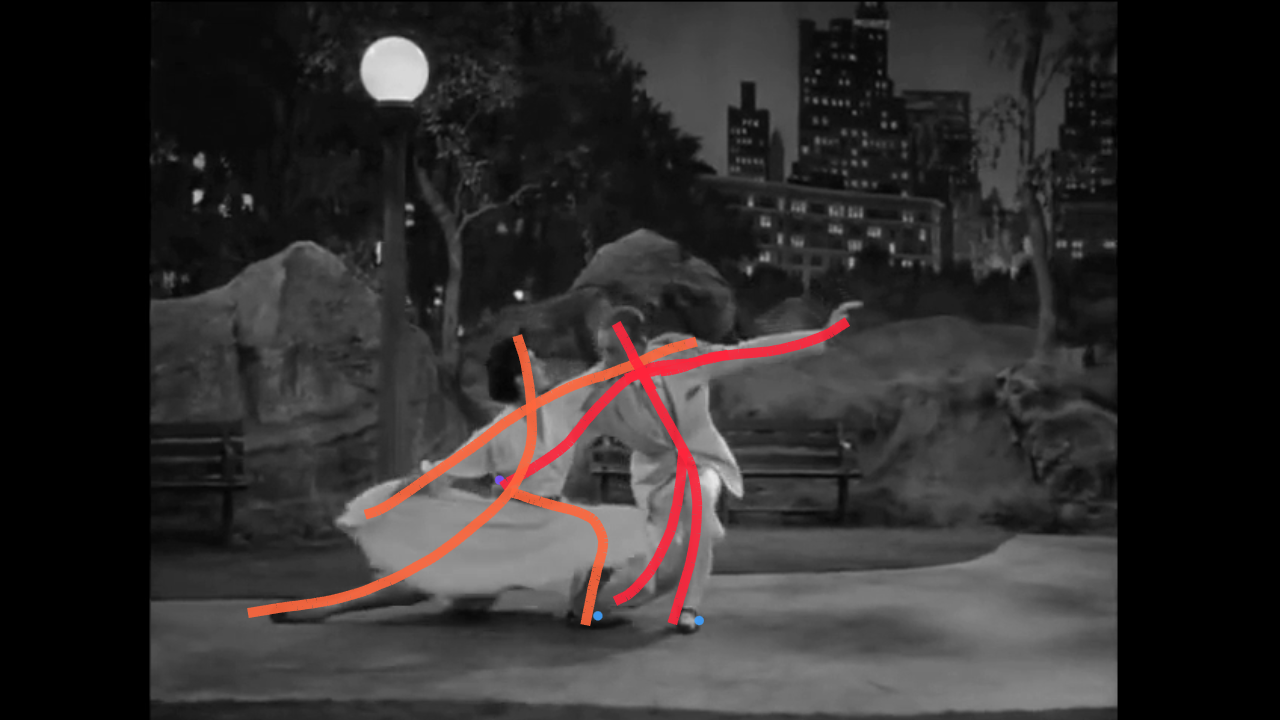
\includegraphics[width=\linewidth]{img/keyframe_case_7_baseline}
                \caption{The typical lines of action trace out the whole skeleton like Sutton notation, and in the worst case is 3 lines per character. This may not seem like such an overwhelming amount, but keeping consistency through a whole clip is cumbersome.}
                \label{fig:baseline}
        \end{subfigure}
        \quad
        \begin{subfigure}[b!]{0.45\textwidth}
        	\centering
                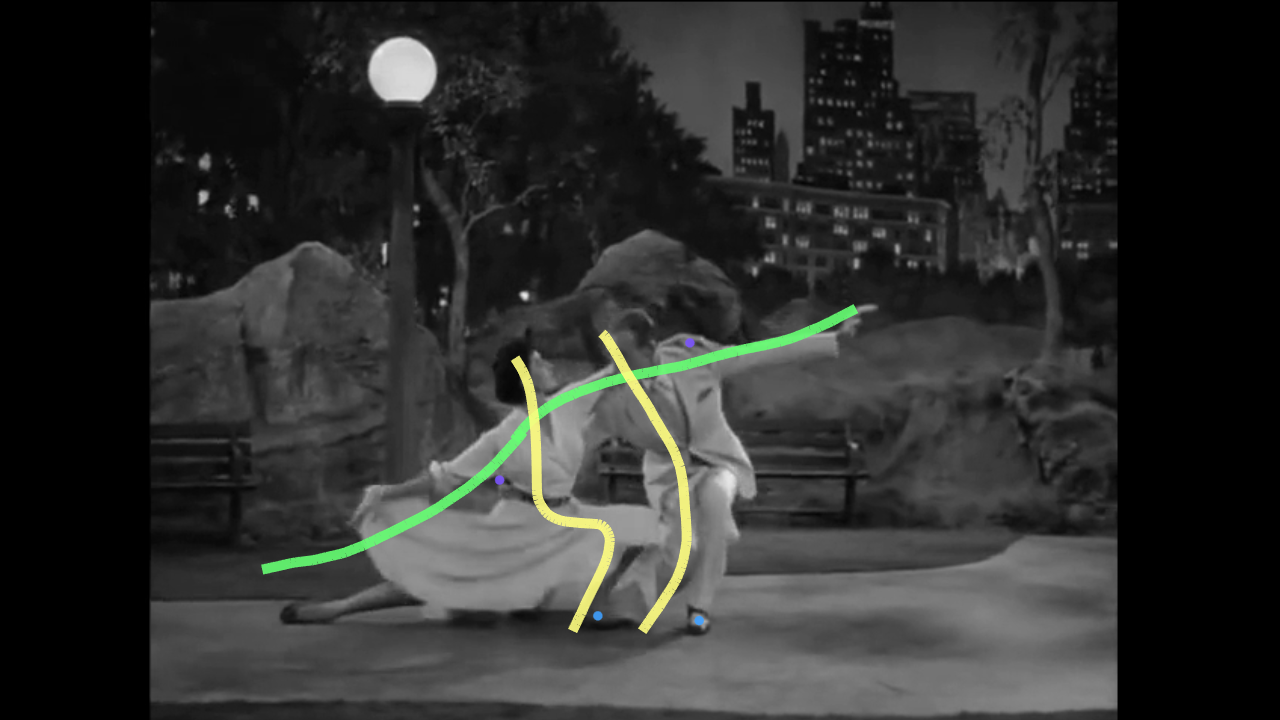
\includegraphics[width=\linewidth]{img/keyframe_case_7_new}
                \caption{Treating the dancers as one character allows the user to draw fewer lines to indicate the same pose. LOAs indicate position and orientation, so the secondary line in green controls both the arm and leg on the left.}
                \label{fig:new_notation}
        \end{subfigure}%
        \caption{Comparing the old line of action and the new.}
	\label{fig:poses}
\end{figure}

Through this process, certain patterns and common poses emerged, enabling the development of an improved notation for illustrating the poses of characters during their interactions with each other. Patterns included symmetry, parallelism, and repetition. Of course, using these patterns and assumptions to our advantage is what drove the development of a solution. It seemed that during many instances in the clip, it would be more efficient to draw lines over the two dancers as if they were one character. This morphed ``combined'' character should be easier to pose and animate.

\begin{figure}[h!]
	\centering
        \begin{subfigure}[b!]{0.31\textwidth}
        	\centering
                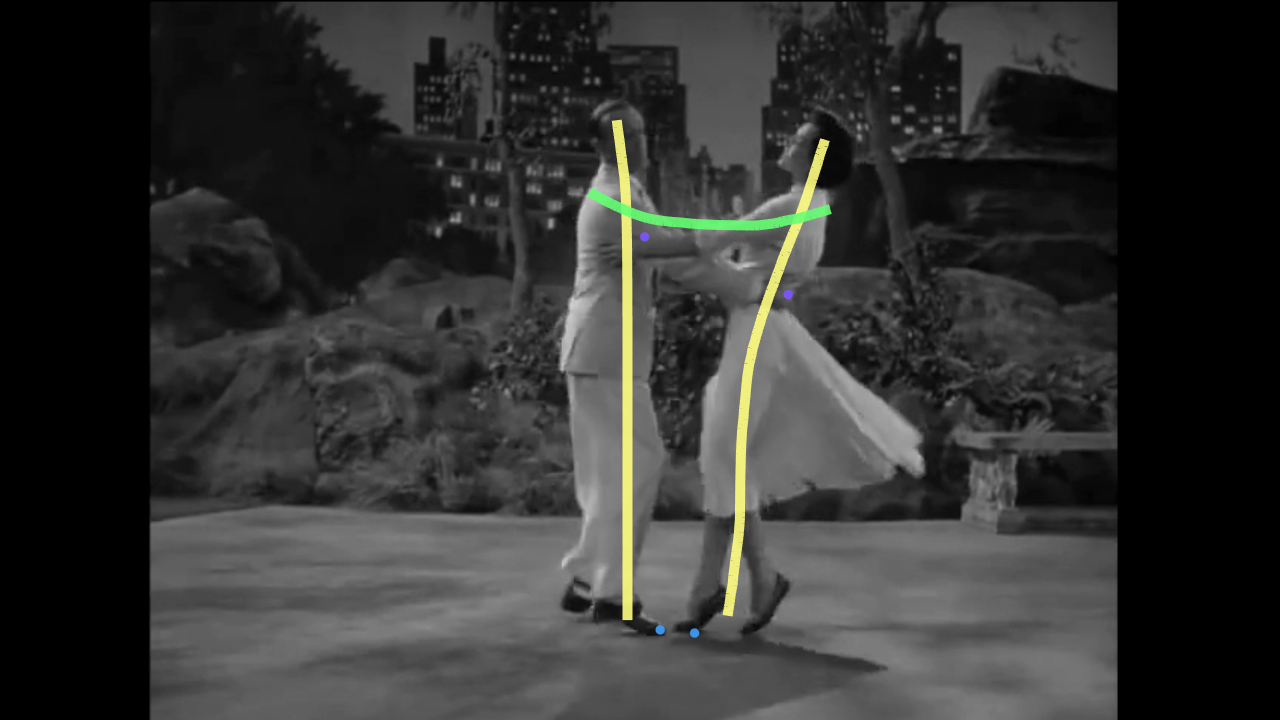
\includegraphics[width=\linewidth]{img/keyframe_case_4_(3)}
                \label{fig:pose1}
        \end{subfigure}
        \quad
        \begin{subfigure}[b!]{0.31\textwidth}
        	\centering
                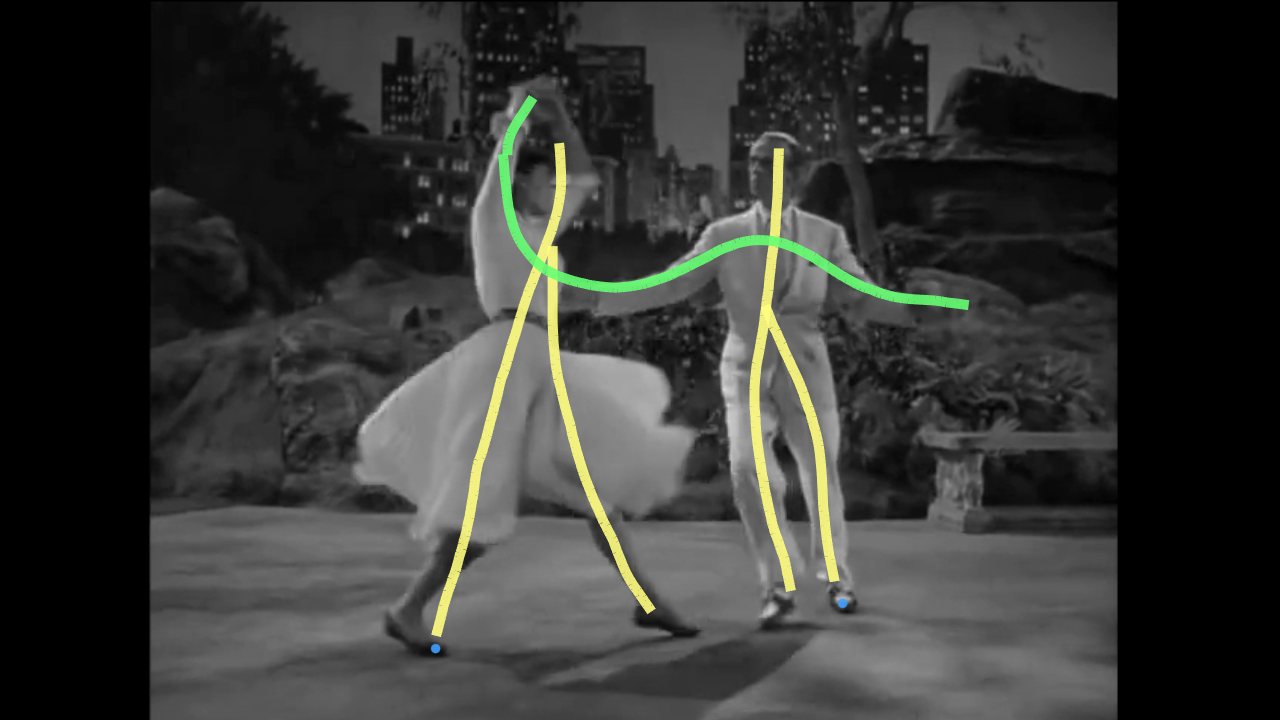
\includegraphics[width=\linewidth]{img/keyframe_case_10_(5)}
                \label{fig:pose2}
        \end{subfigure}%
        \quad
        \begin{subfigure}[b!]{0.31\textwidth}
        	\centering
                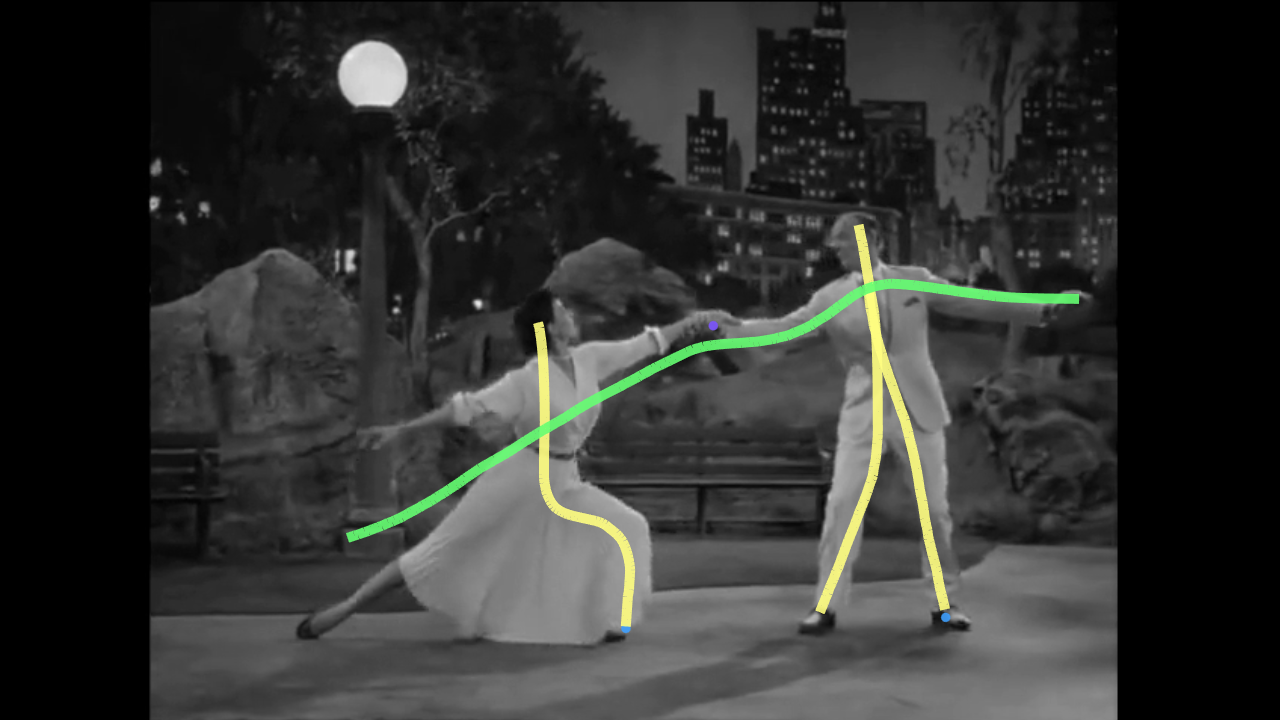
\includegraphics[width=\linewidth]{img/keyframe_case_7_(4)}
                \label{fig:pose3}
        \end{subfigure}%
	\caption{A selection of tracings over the dance clip from ``The Band Wagon.''}
	\label{fig:tracing}
\end{figure}

\subsection{Notation}
Taking inspiration from Sutton Notation, we propose a new notation for representing the poses of two characters both together and separately.

There is a dance scene in the film ``The Band Wagon,'' where Cyd Charisse and Fred Astaire start out by walking together side by side, exchanging twirls until it morphs completely into a swing style dance. This scene is our use case for inventing a notation which extends seamlessly to more than one character.

\begin{figure}[H]
\centering
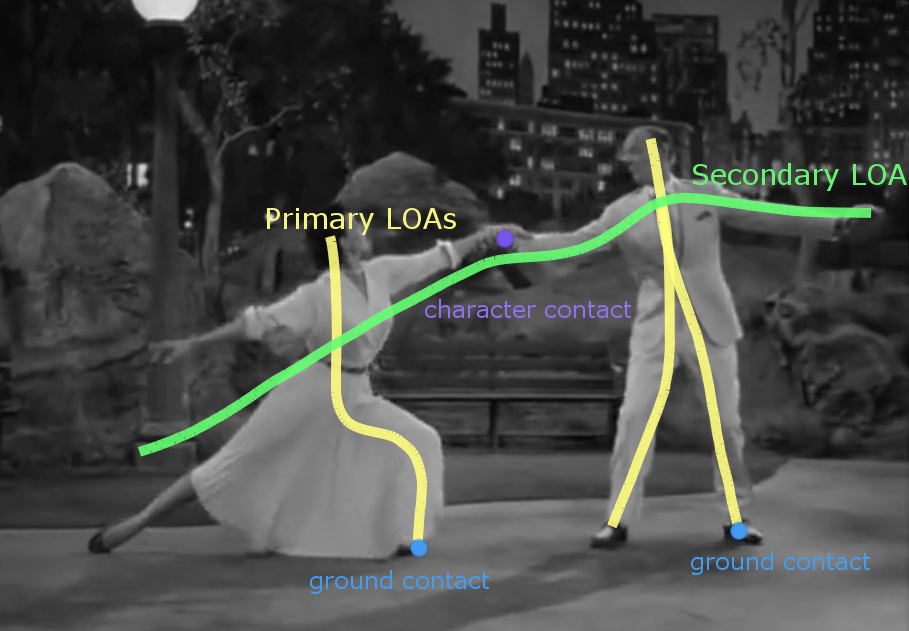
\includegraphics[scale=0.5]{img/labelednotation}
\caption{Labeled notation.}
\end{figure}

To determine which poses for these dancers were common, I annotated the video, keeping track of contact points between the two characters (purple), the contact points with the characters and the ground (blue), the main LOAs (yellow), and the secondary LOAs (green). Once the video was annotated, I categorized the keyframes into how many LOAs it took to create that pose. I chose the most extreme examples of each combination that I could find.
\newpage

\begin{table}[h!]
\centering
\begin{tabular}{ll}
	\begin{minipage}{.28\textwidth}
      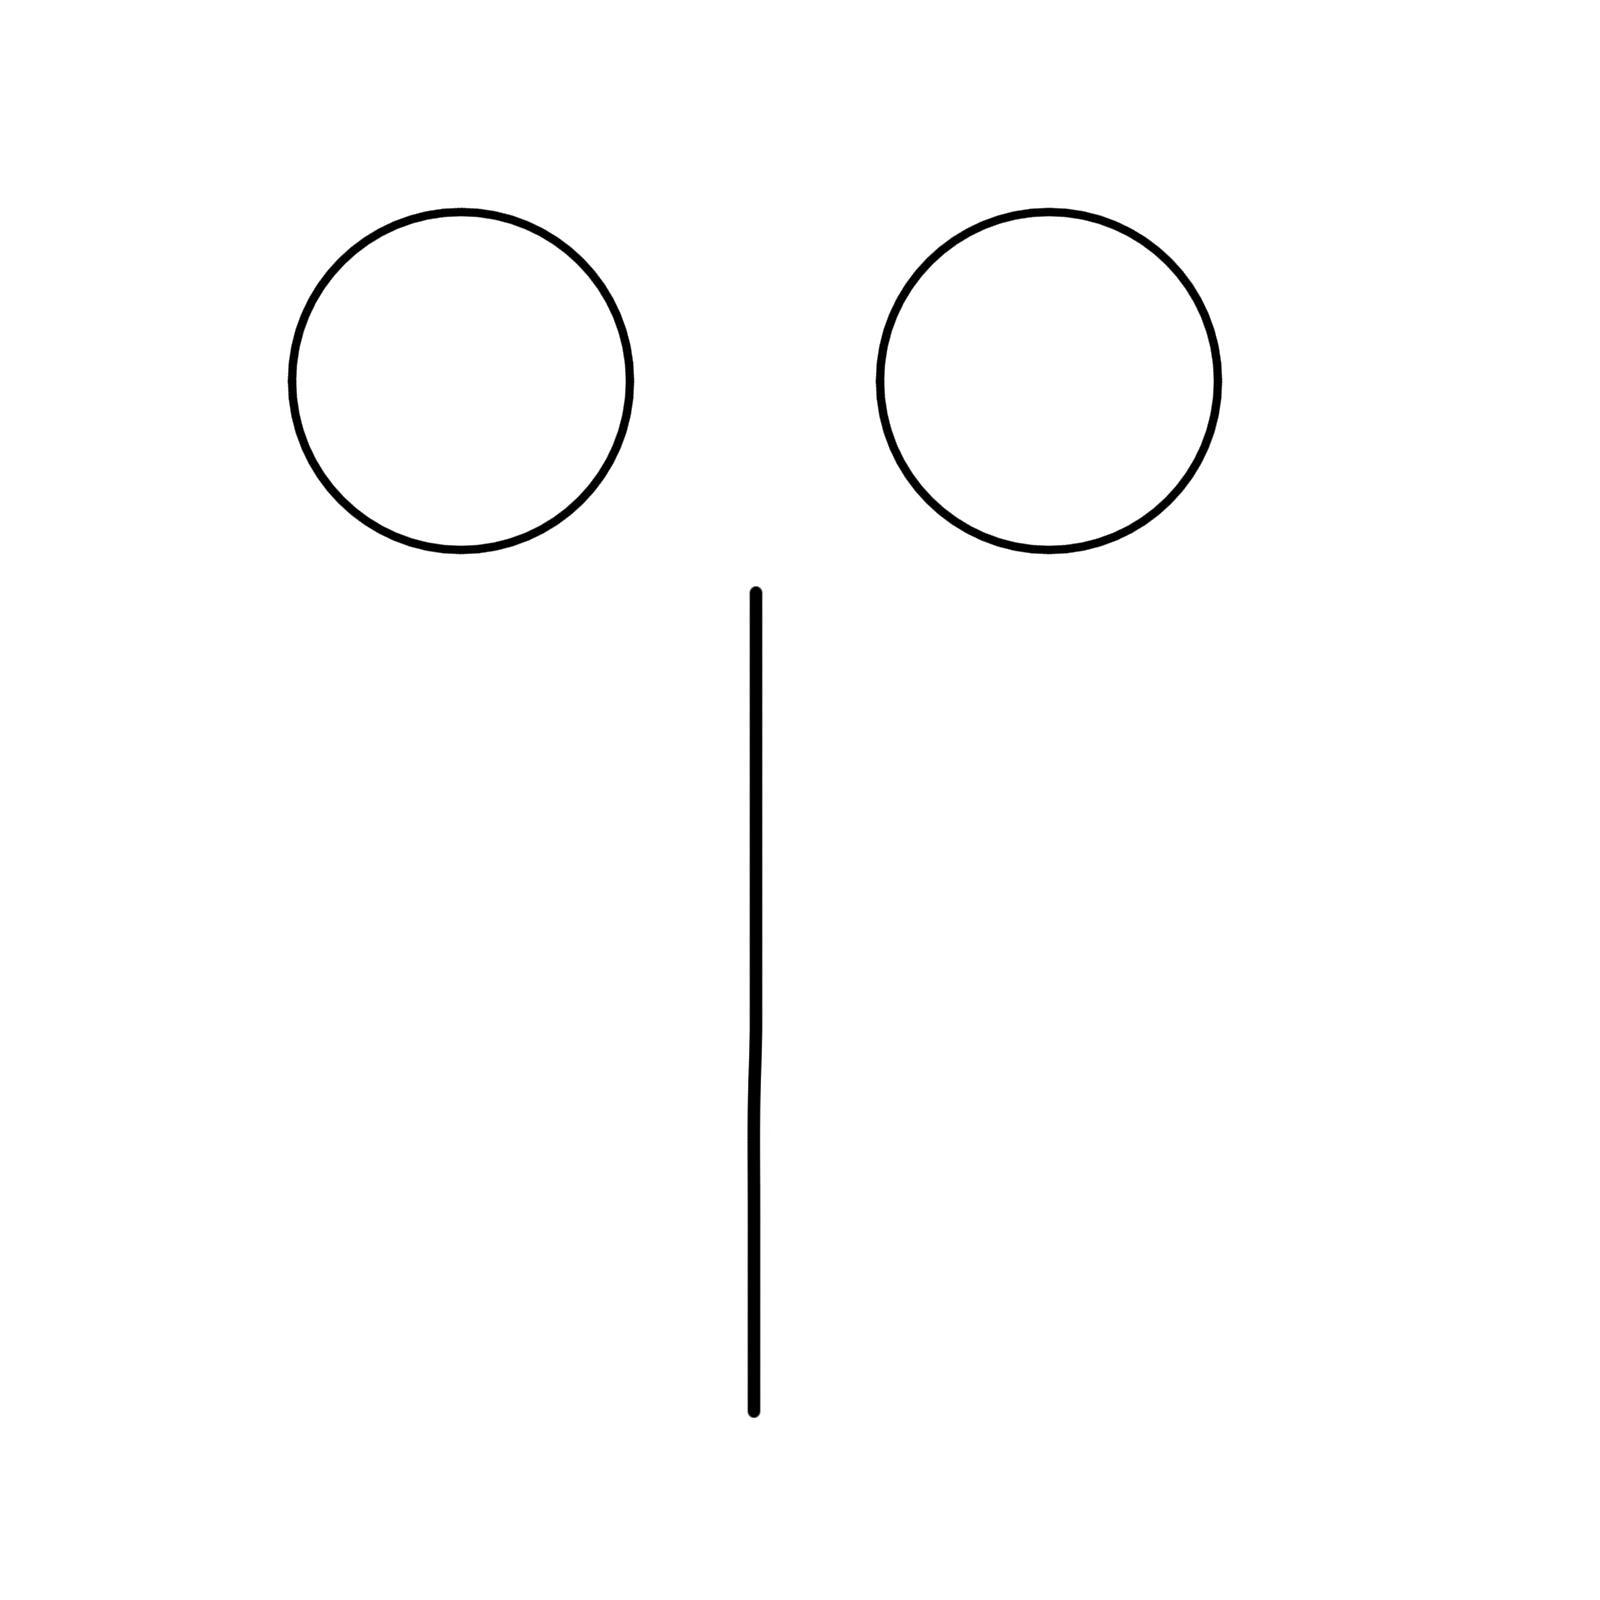
\includegraphics[width=\linewidth, height=25mm]{img/01keyframe}
    \end{minipage} &  
    \begin{minipage}{.28\textwidth}
      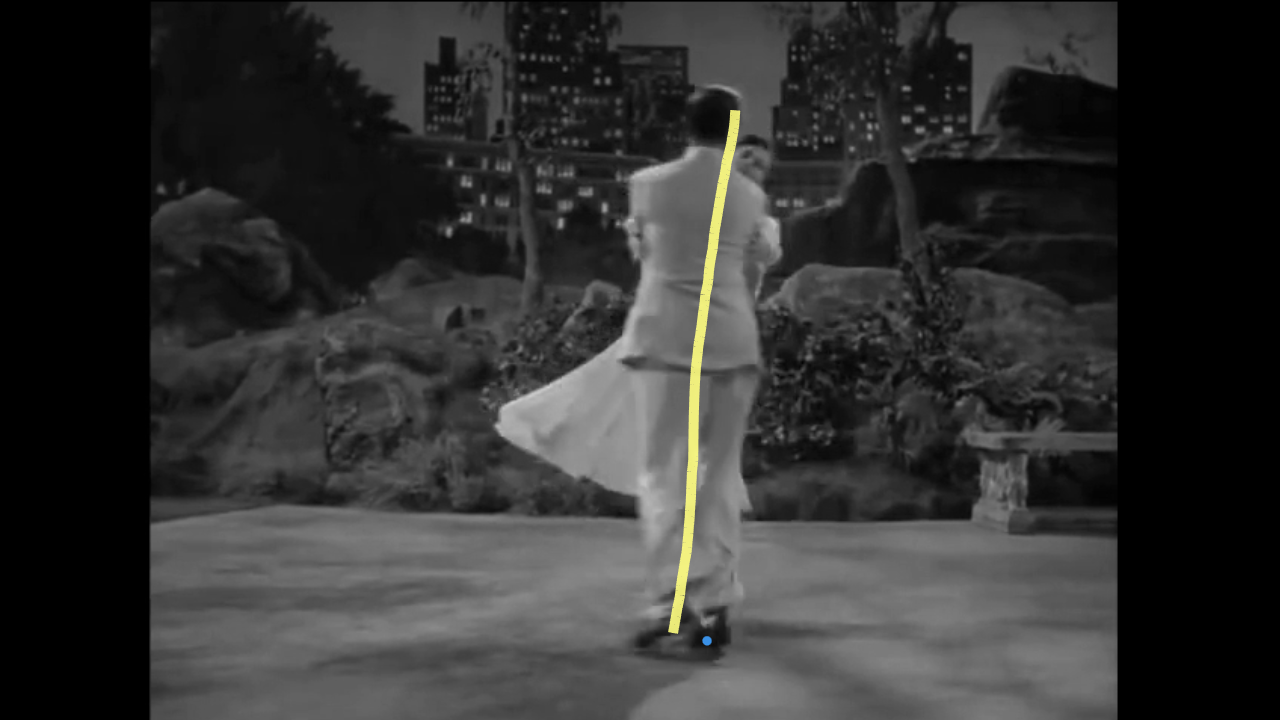
\includegraphics[width=\linewidth, height=25mm]{img/keyframe_case_1_(1)}
    \end{minipage}\\
	\begin{minipage}{.28\textwidth}
      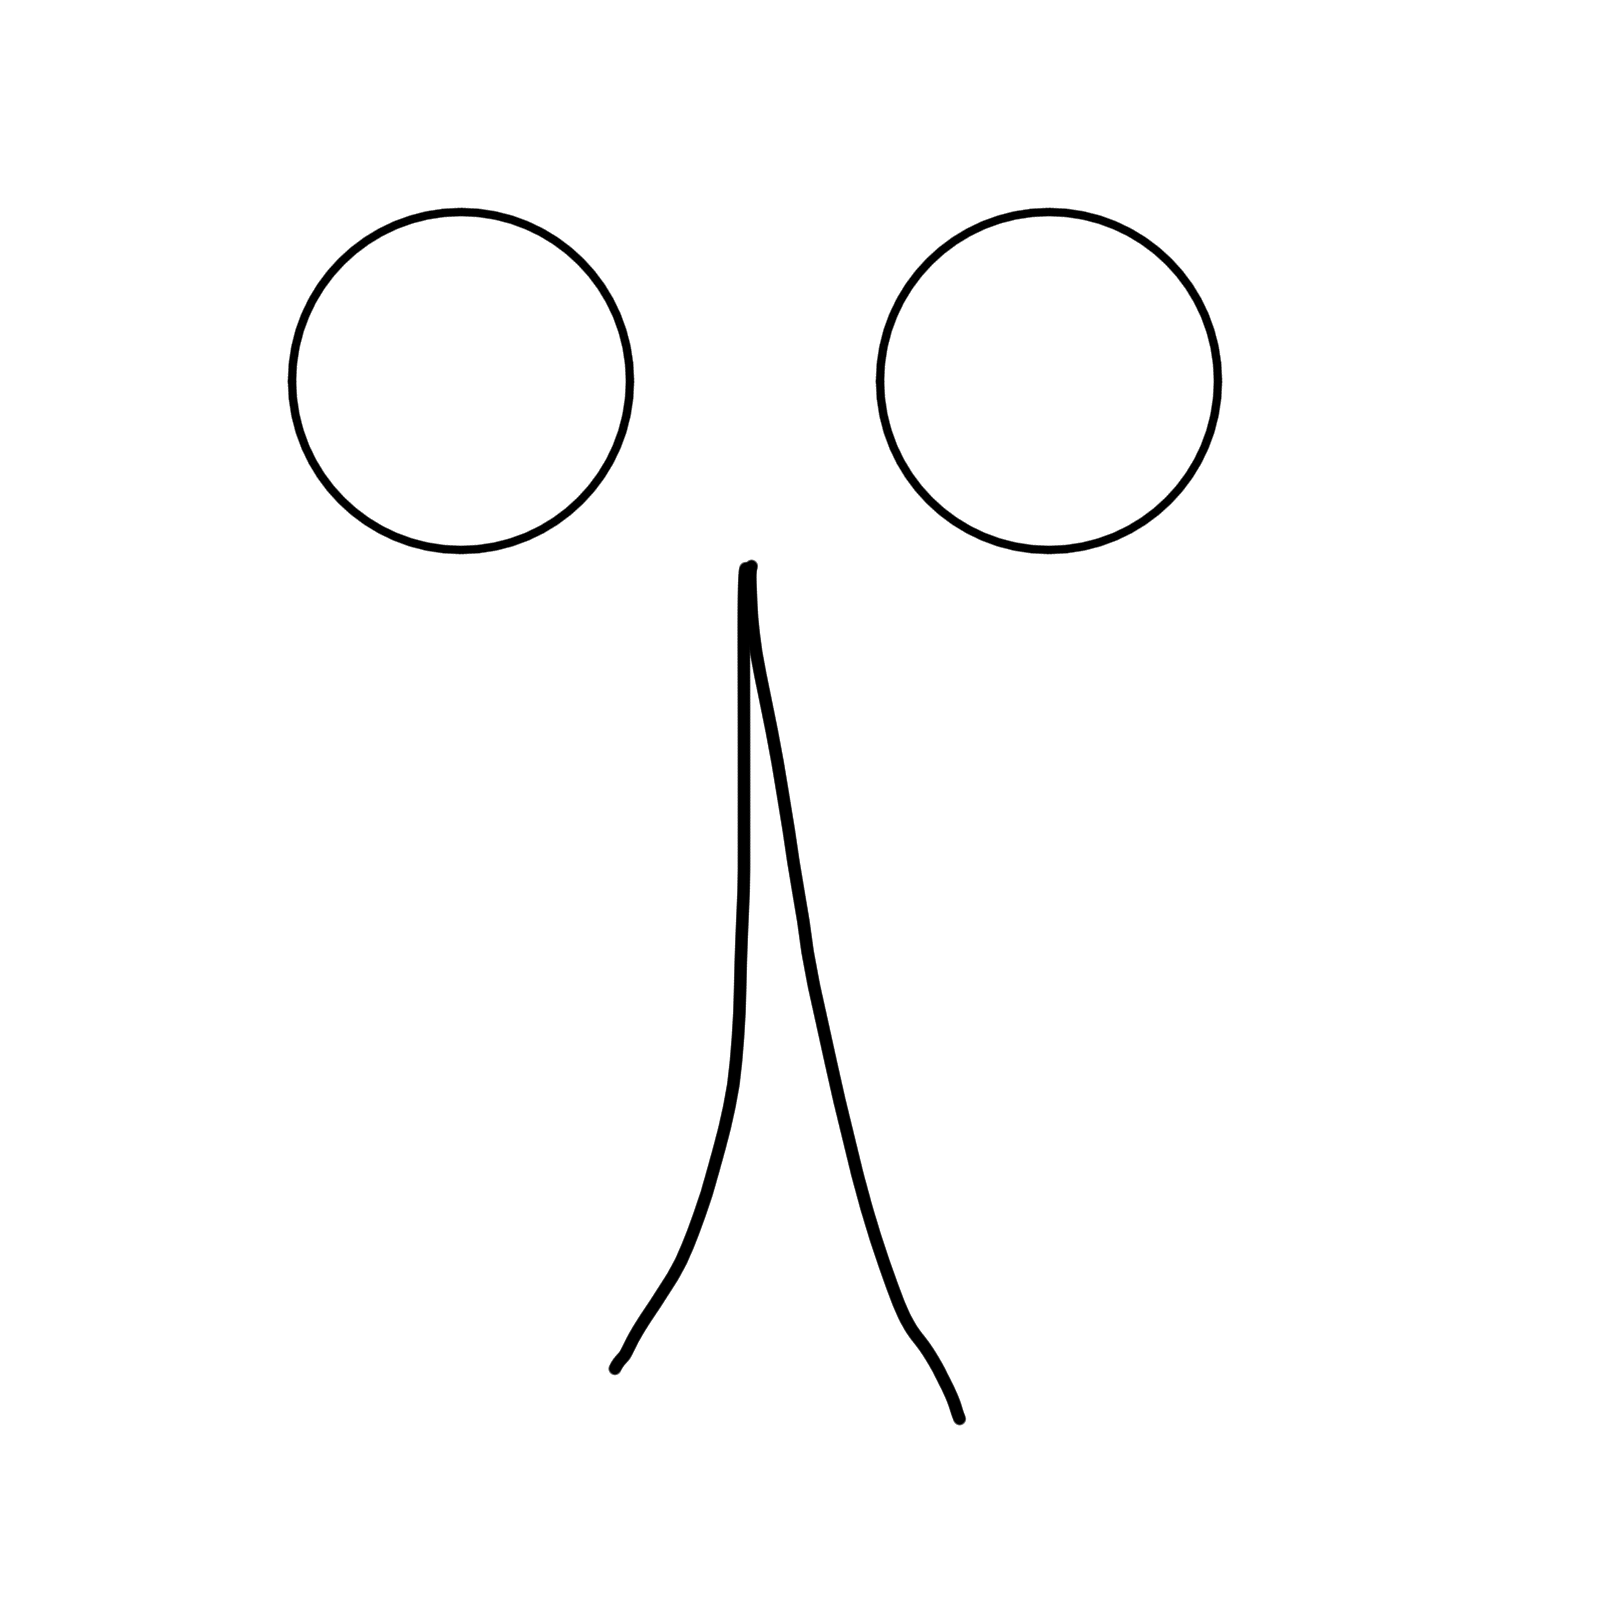
\includegraphics[width=\linewidth, height=25mm]{img/02keyframe}
    \end{minipage} & 
        \begin{minipage}{.28\textwidth}
      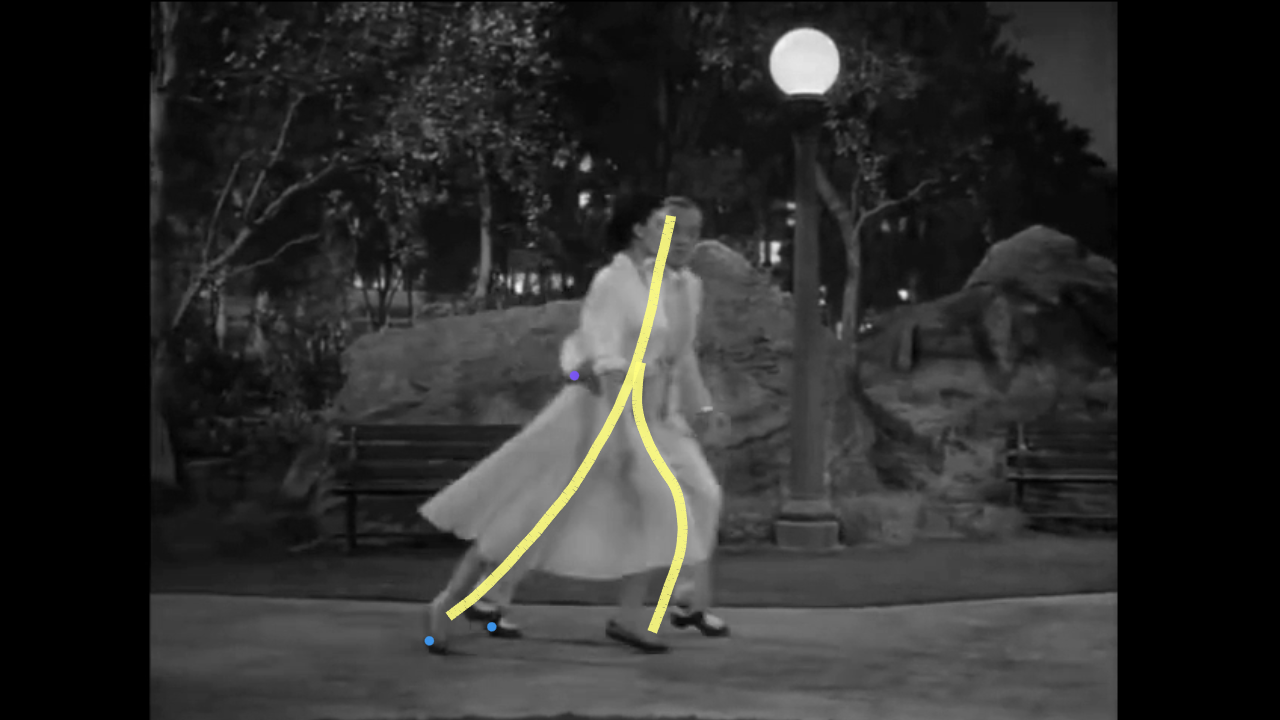
\includegraphics[width=\linewidth, height=25mm]{img/keyframe_case_2_(2)}
    \end{minipage} \\
	\begin{minipage}{.28\textwidth}
      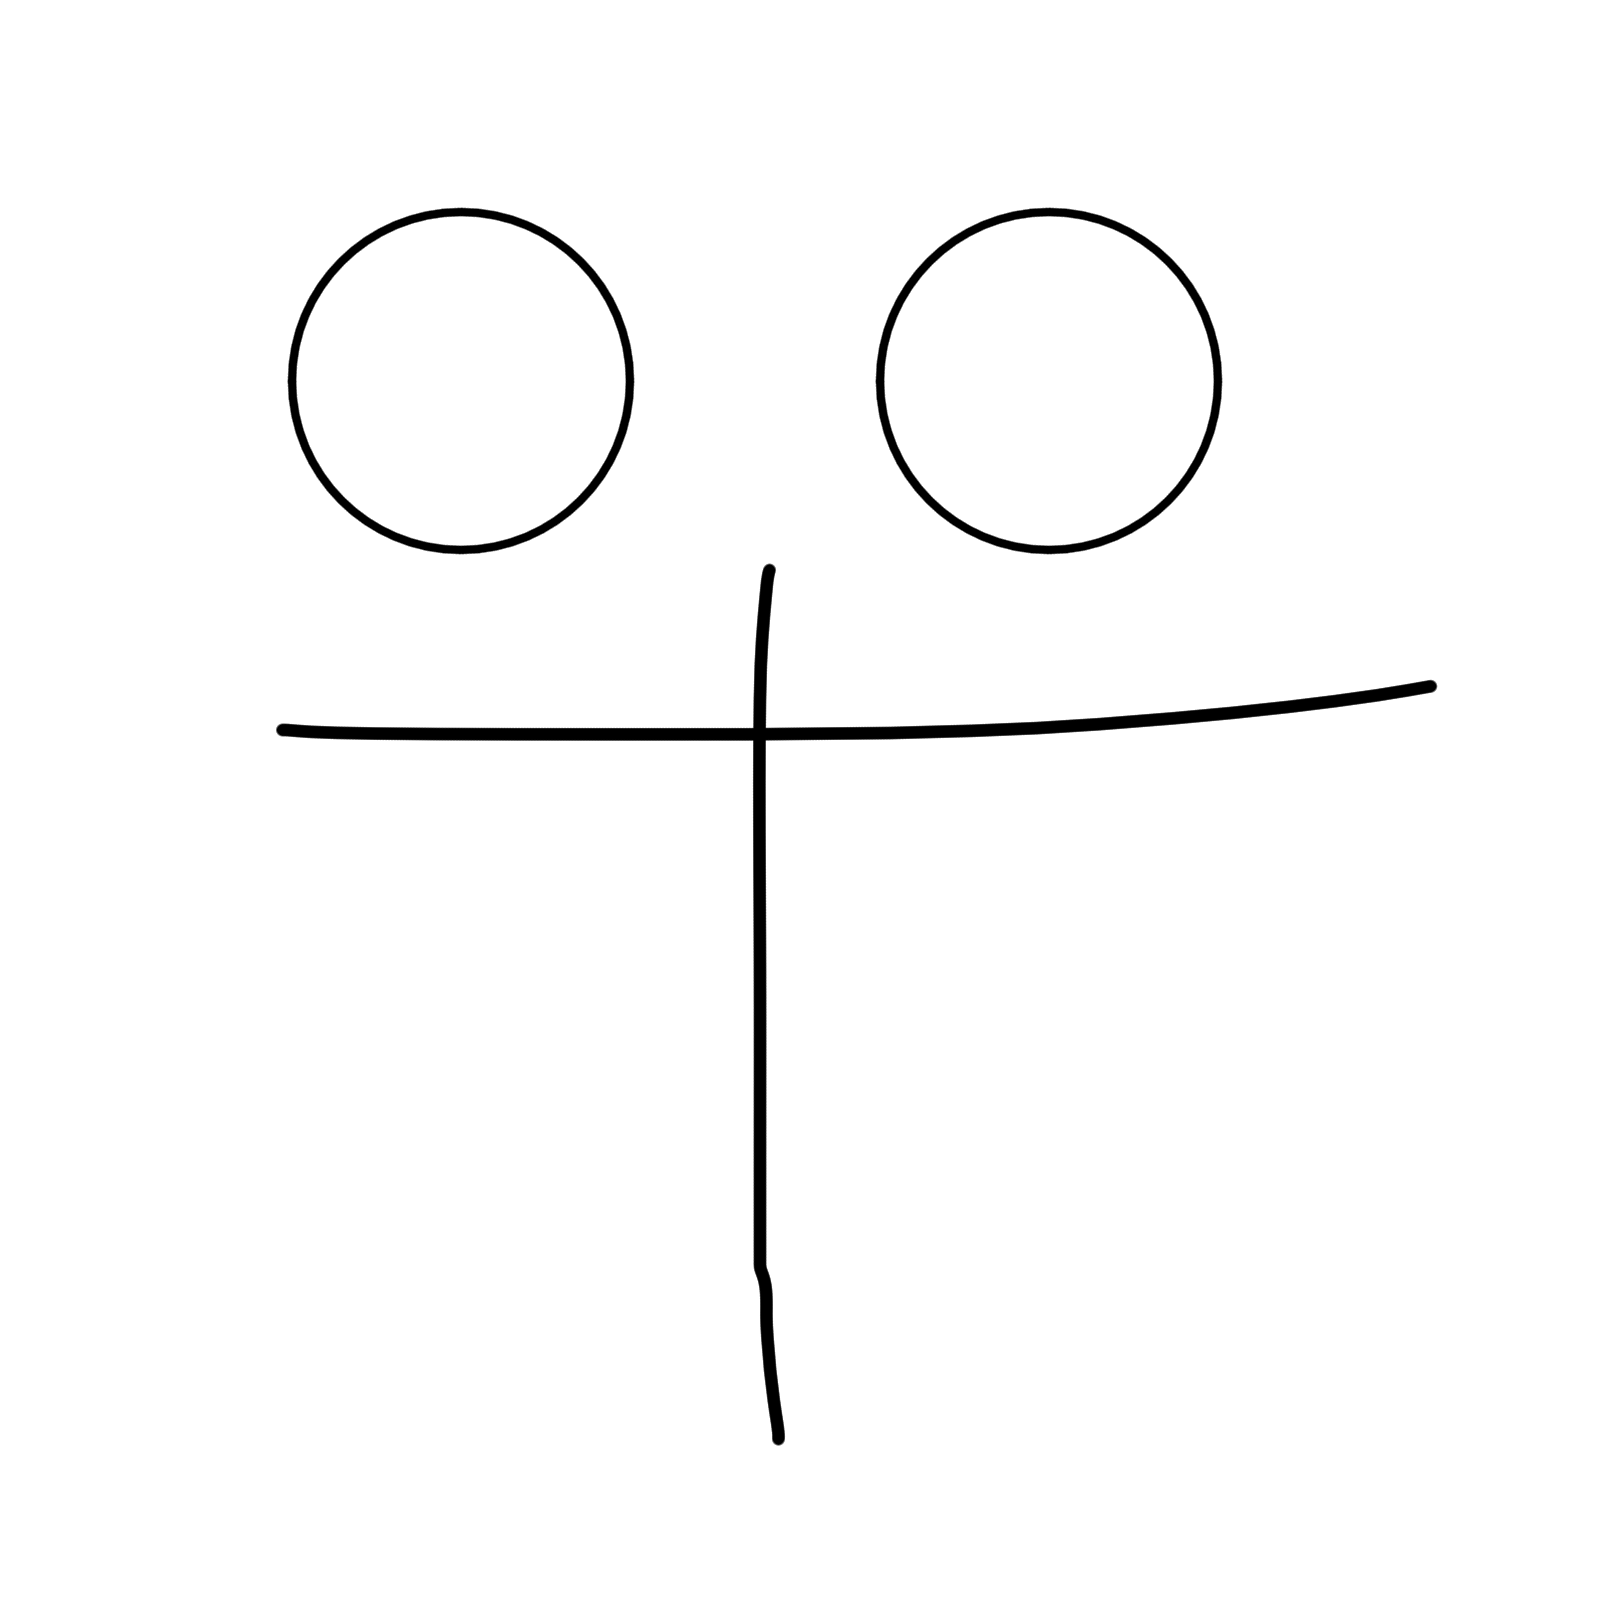
\includegraphics[width=\linewidth, height=25mm]{img/03keyframe}
    \end{minipage} & 
    \begin{minipage}{.28\textwidth}
      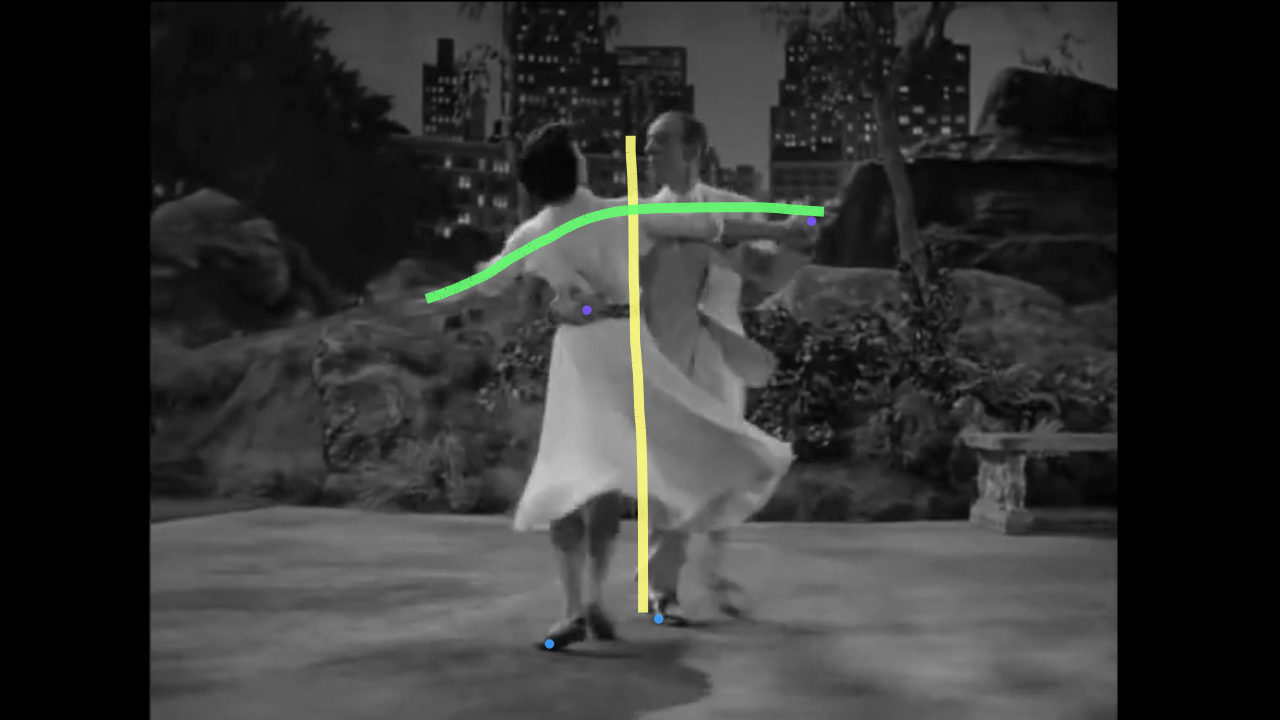
\includegraphics[width=\linewidth, height=25mm]{img/keyframe_case_3_(2)}
    \end{minipage} \\
	\begin{minipage}{.28\textwidth}
      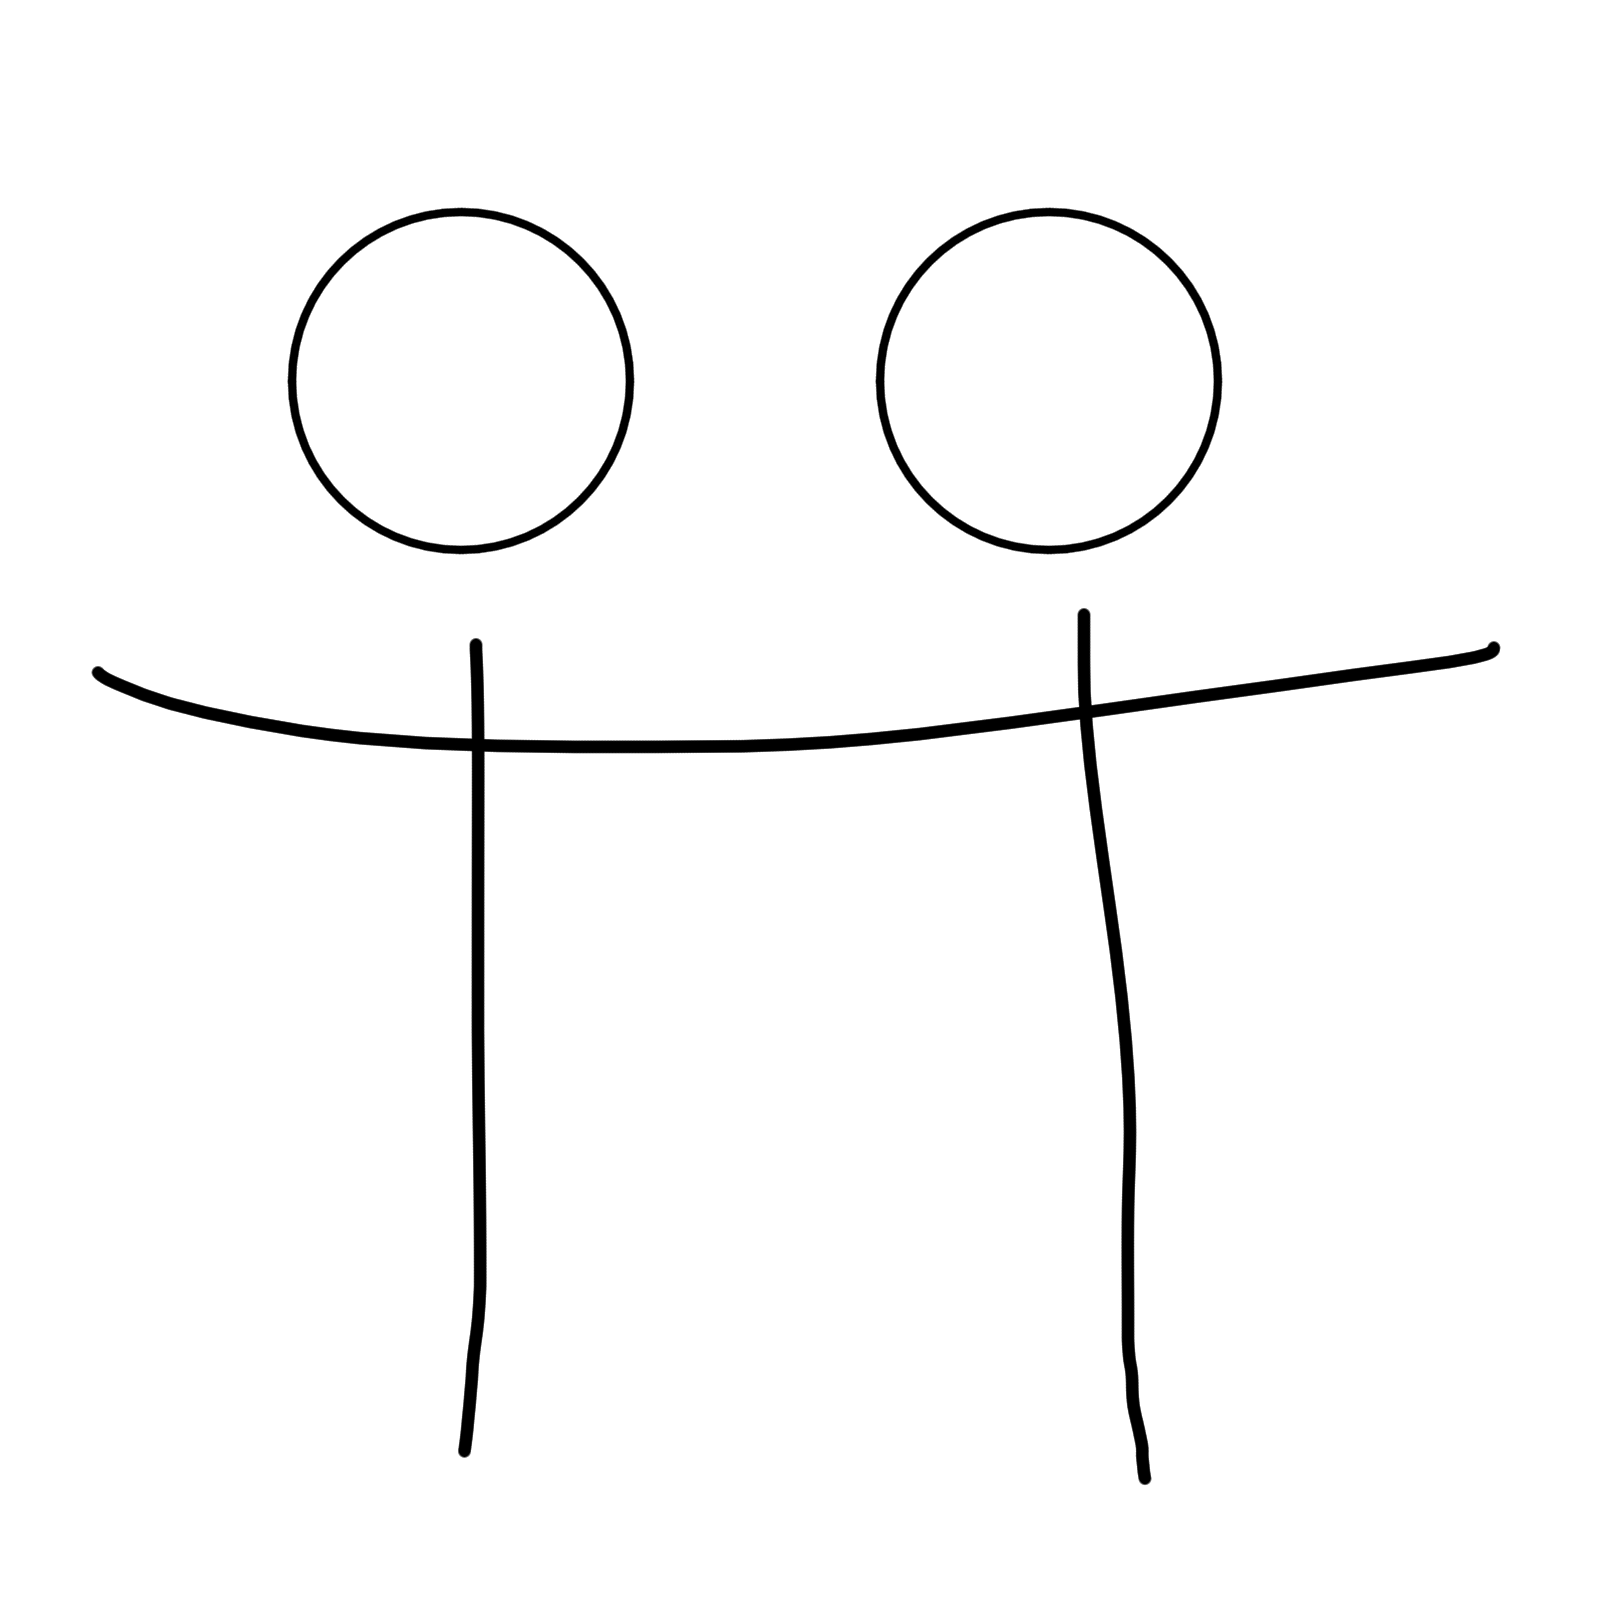
\includegraphics[width=\linewidth, height=25mm]{img/04keyframe}
    \end{minipage} &
    \begin{minipage}{.28\textwidth}
      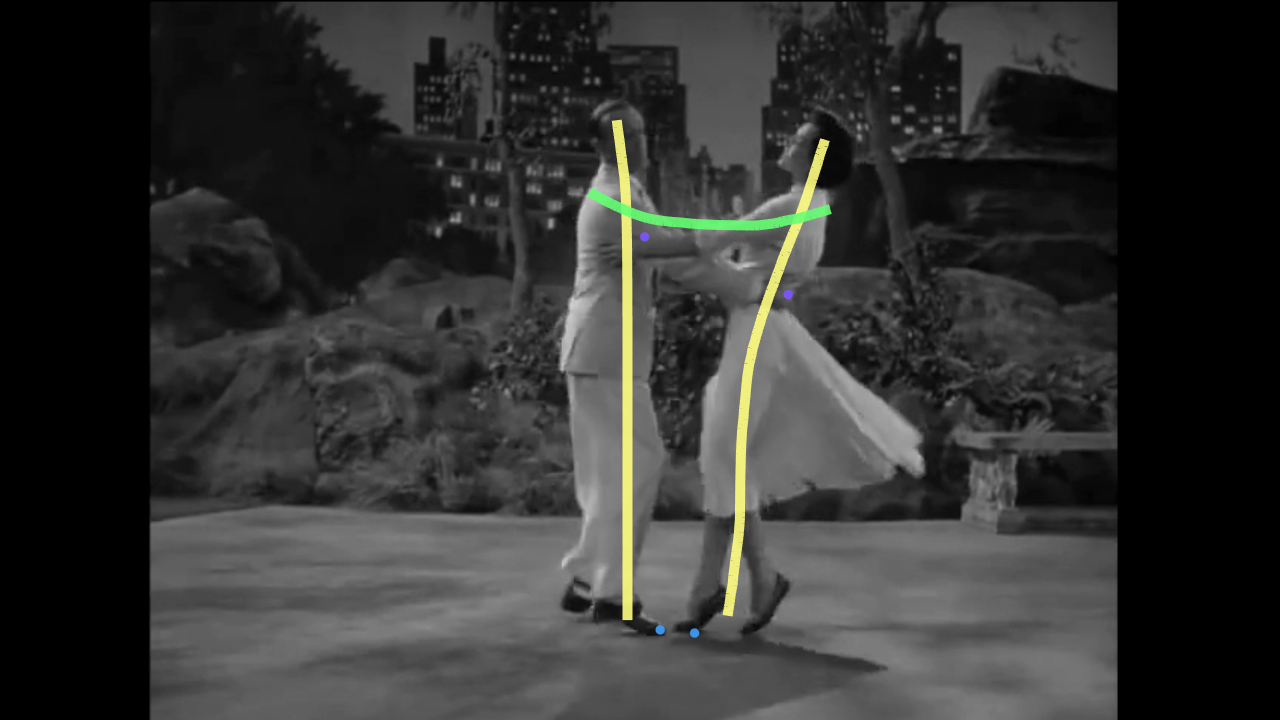
\includegraphics[width=\linewidth, height=25mm]{img/keyframe_case_4_(3)}
    \end{minipage}  \\
	\begin{minipage}{.28\textwidth}
      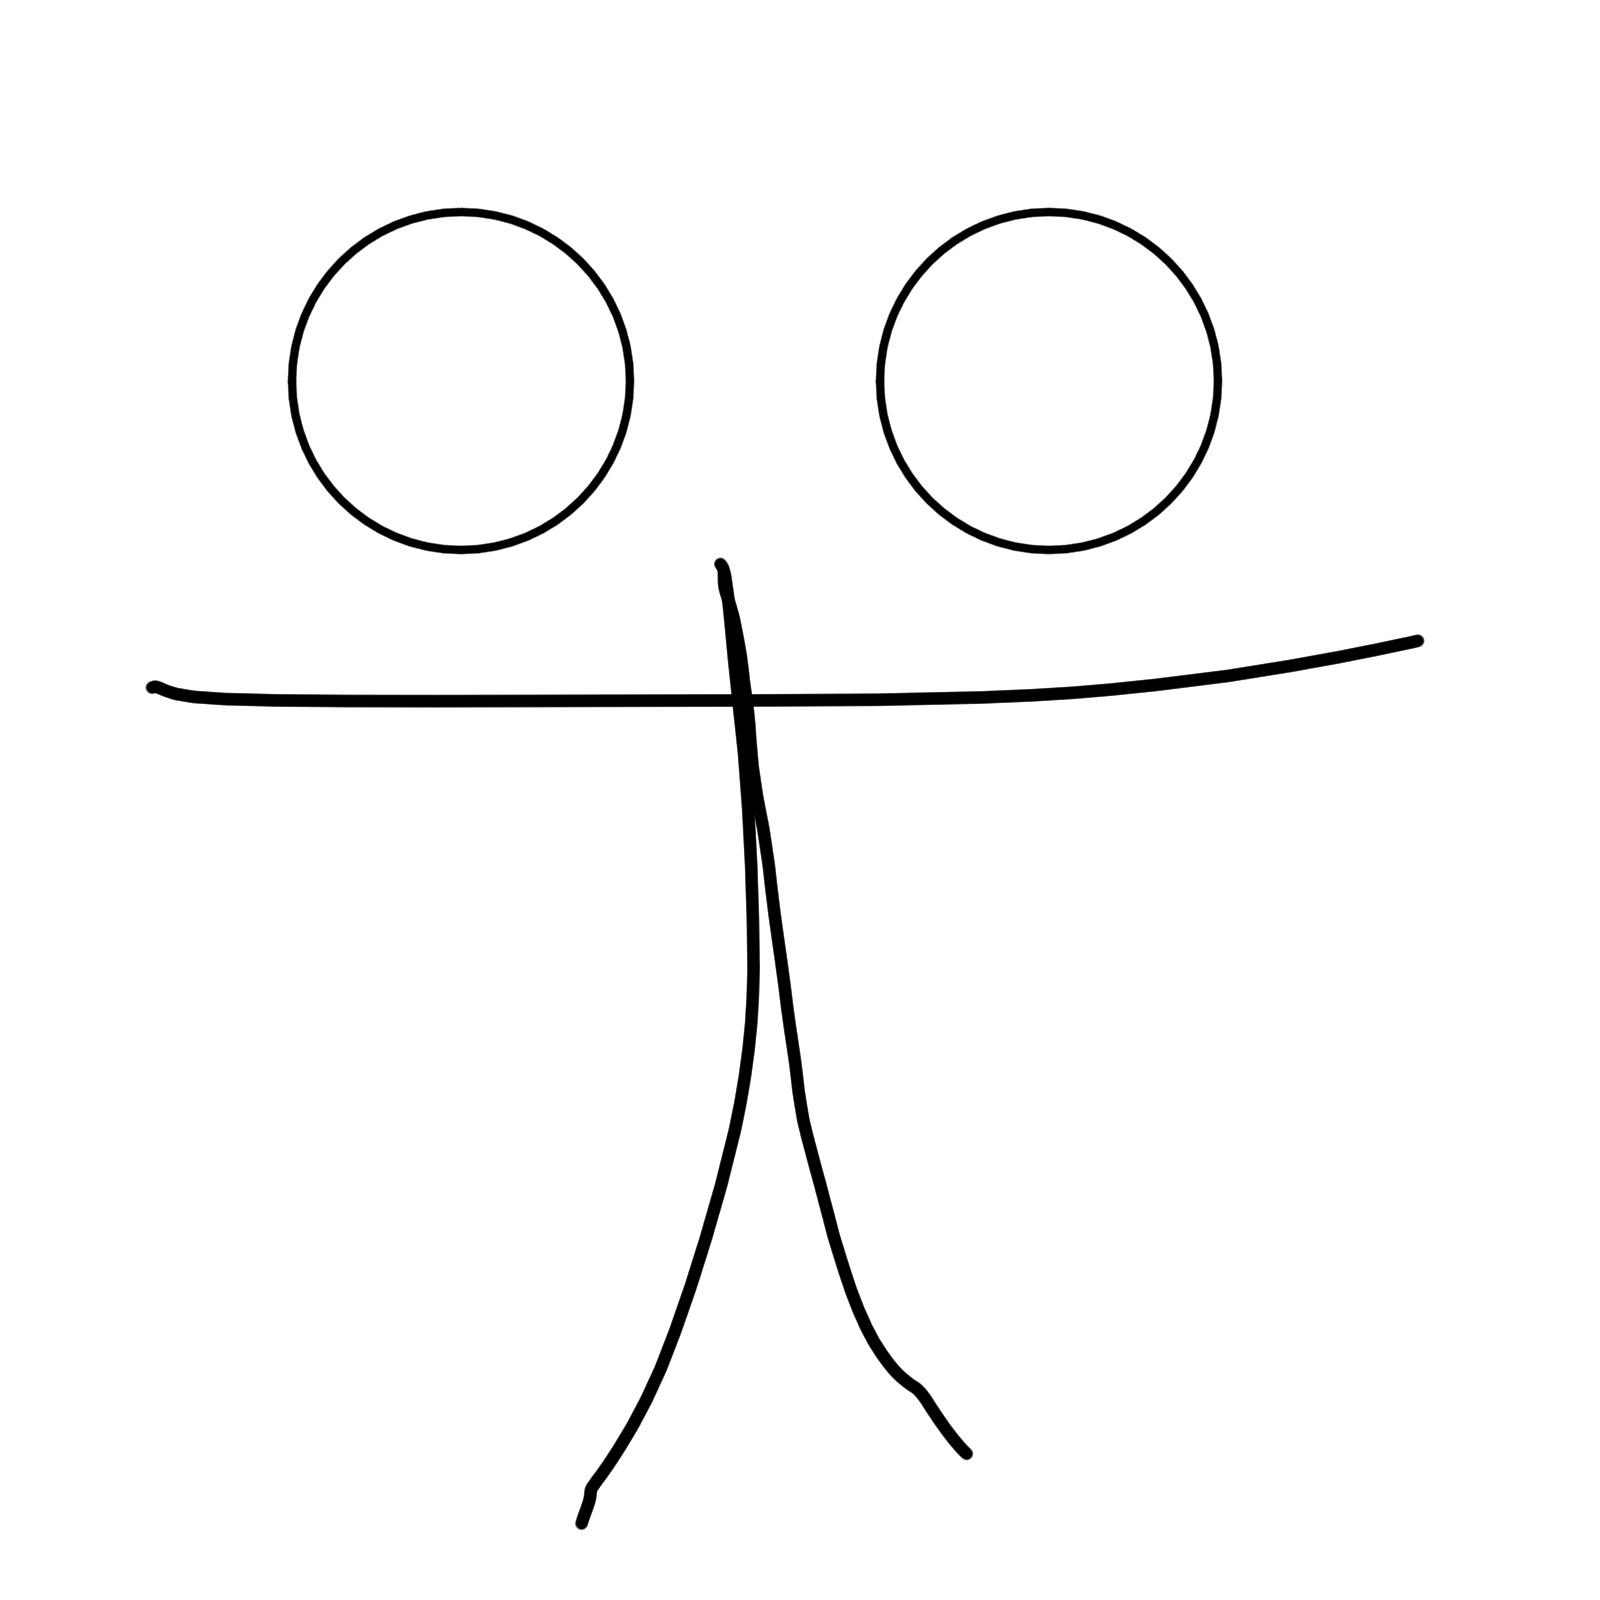
\includegraphics[width=\linewidth, height=25mm]{img/05keyframe}
    \end{minipage} &  
    \begin{minipage}{.28\textwidth}
      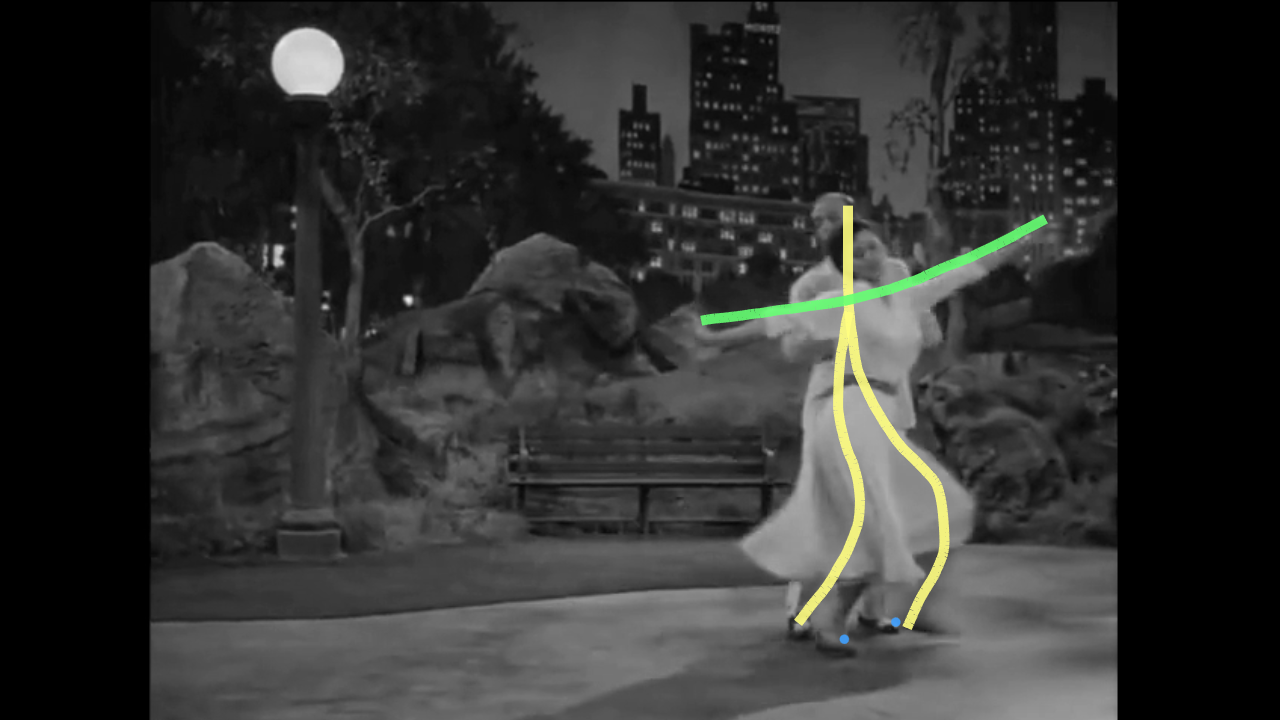
\includegraphics[width=\linewidth, height=25mm]{img/keyframe_case_5_(3)}
    \end{minipage}\\
	\begin{minipage}{.28\textwidth}
      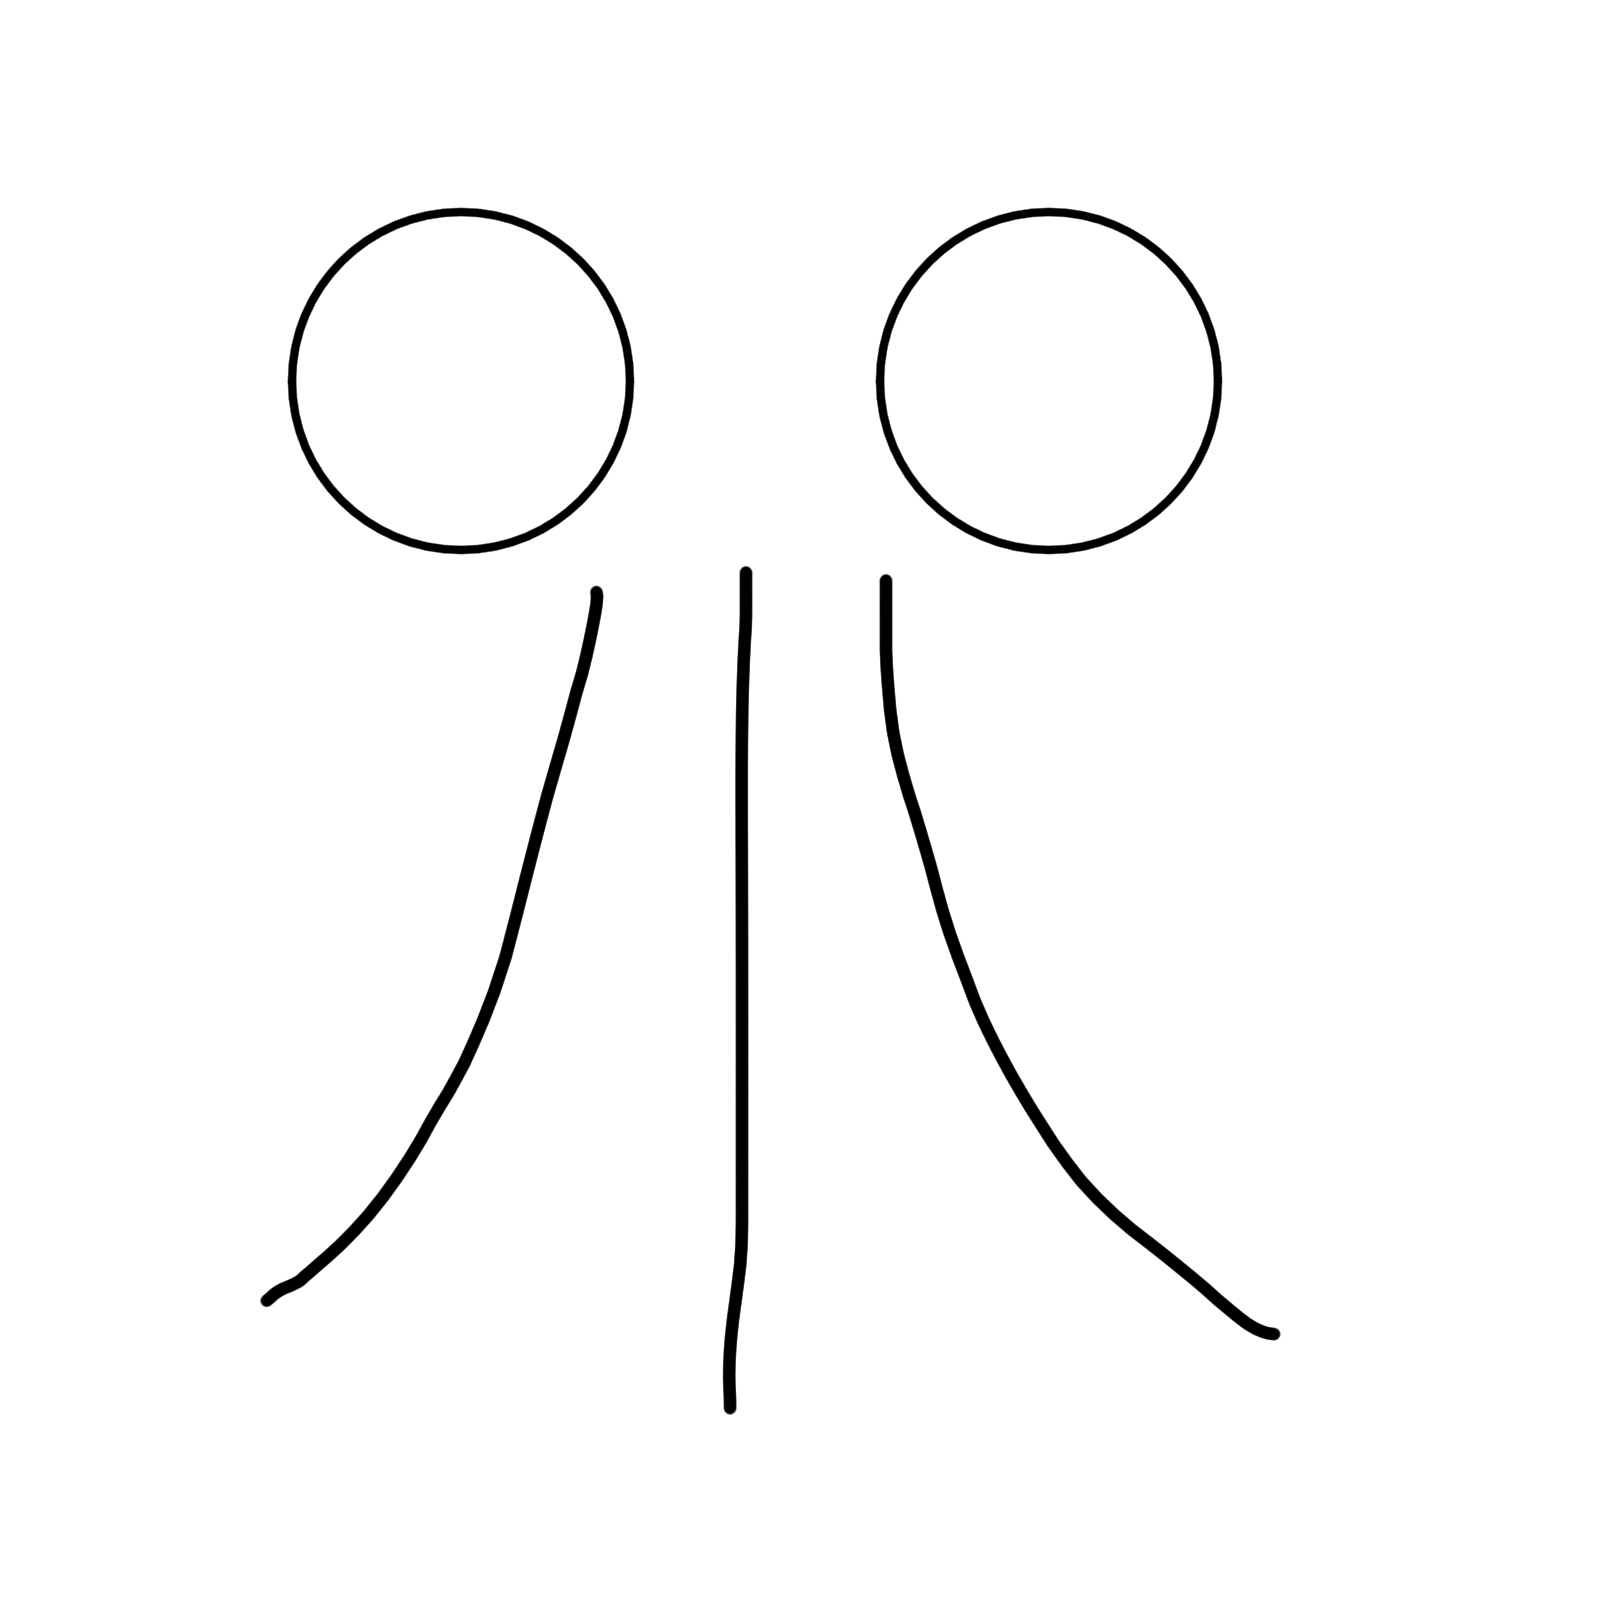
\includegraphics[width=\linewidth, height=25mm]{img/06keyframe}
    \end{minipage} & 
    \begin{minipage}{.28\textwidth}
      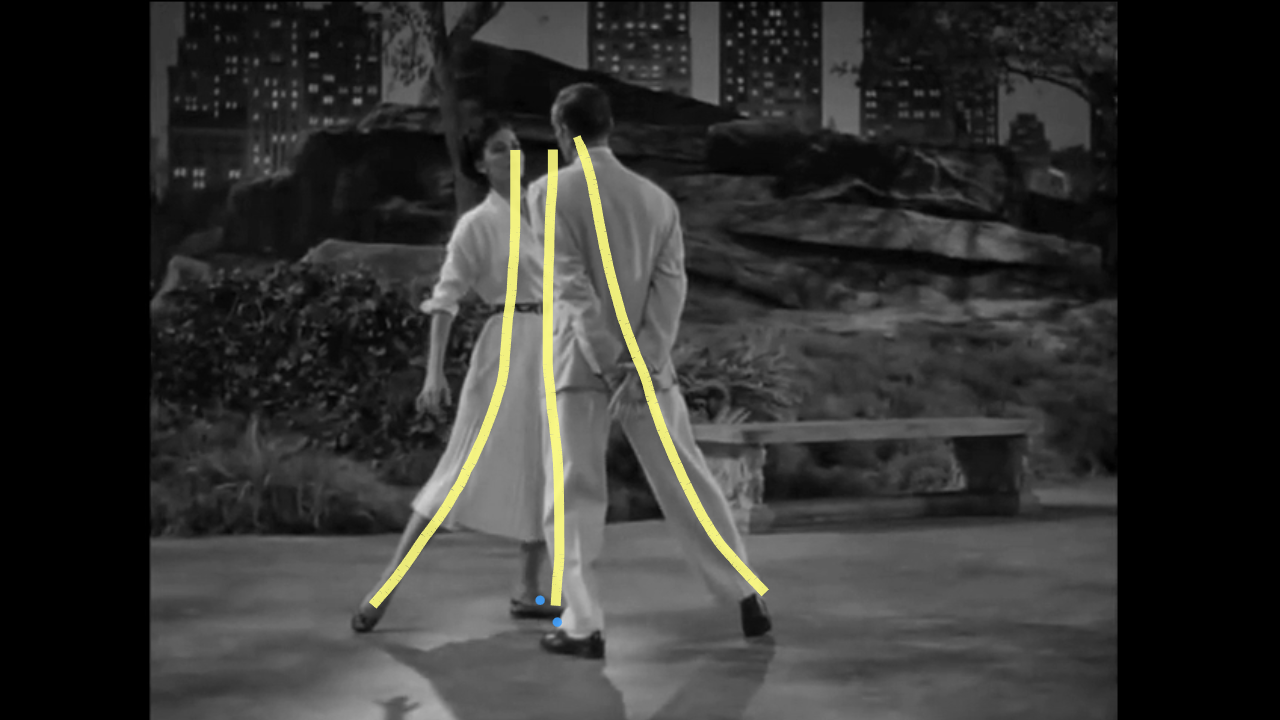
\includegraphics[width=\linewidth, height=25mm]{img/keyframe_case_6_(3)}
    \end{minipage} \\
	\begin{minipage}{.28\textwidth}
      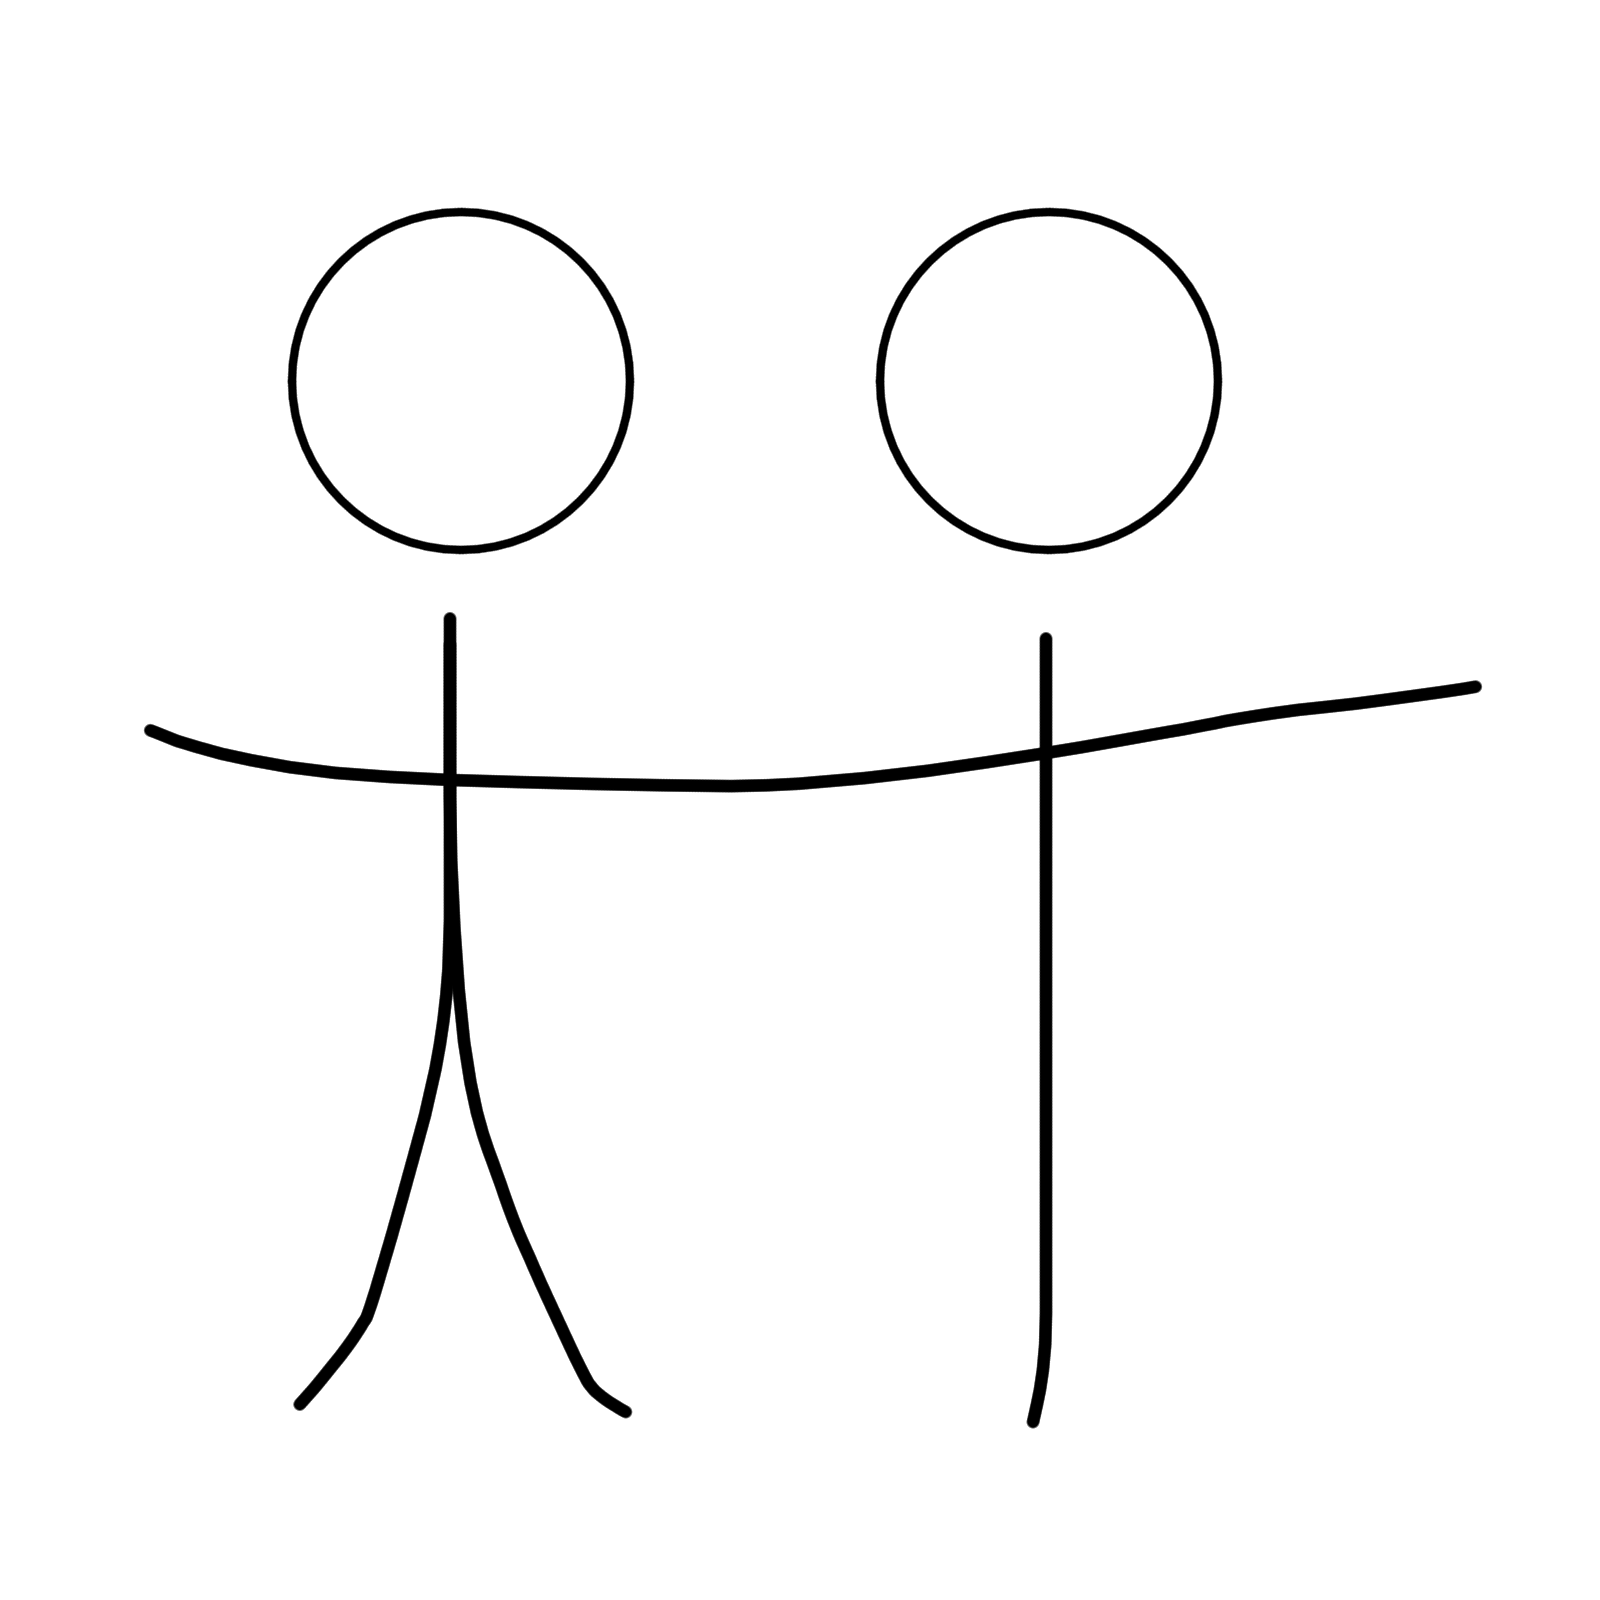
\includegraphics[width=\linewidth, height=25mm]{img/07keyframe}
    \end{minipage} &  
    \begin{minipage}{.28\textwidth}
      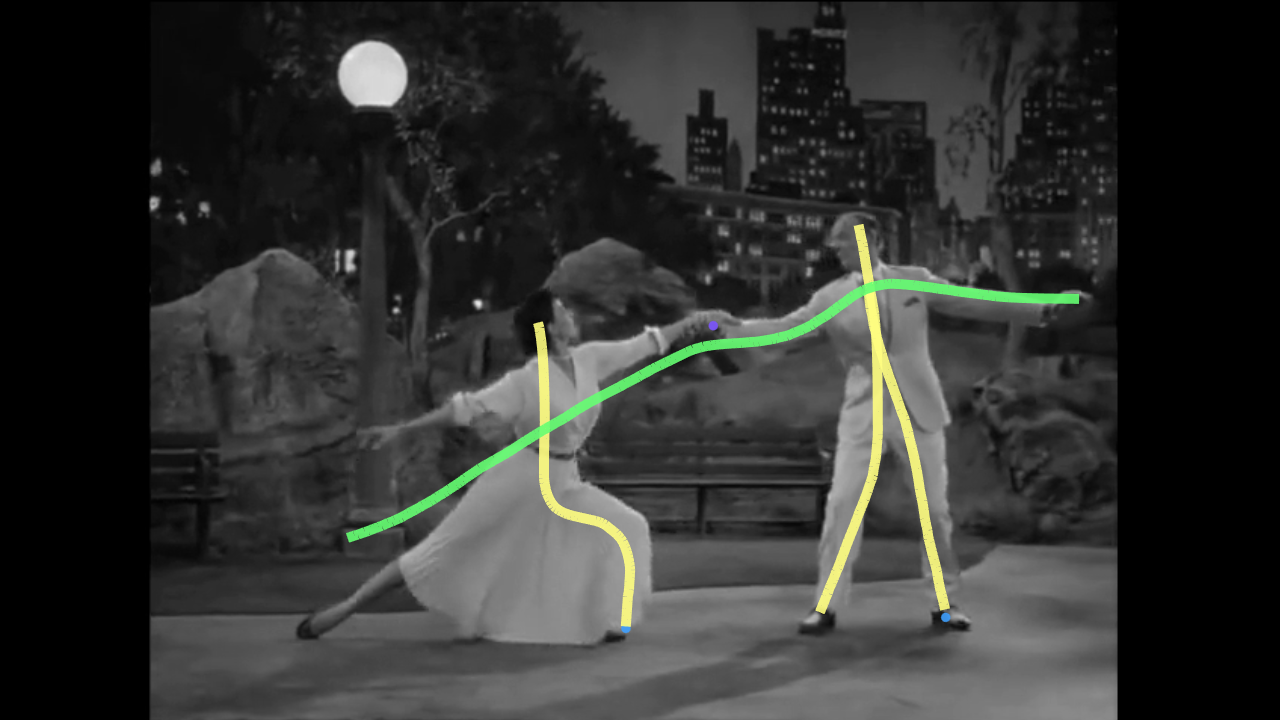
\includegraphics[width=\linewidth, height=25mm]{img/keyframe_case_7_(4)}
    \end{minipage}\\
	\begin{minipage}{.28\textwidth}
      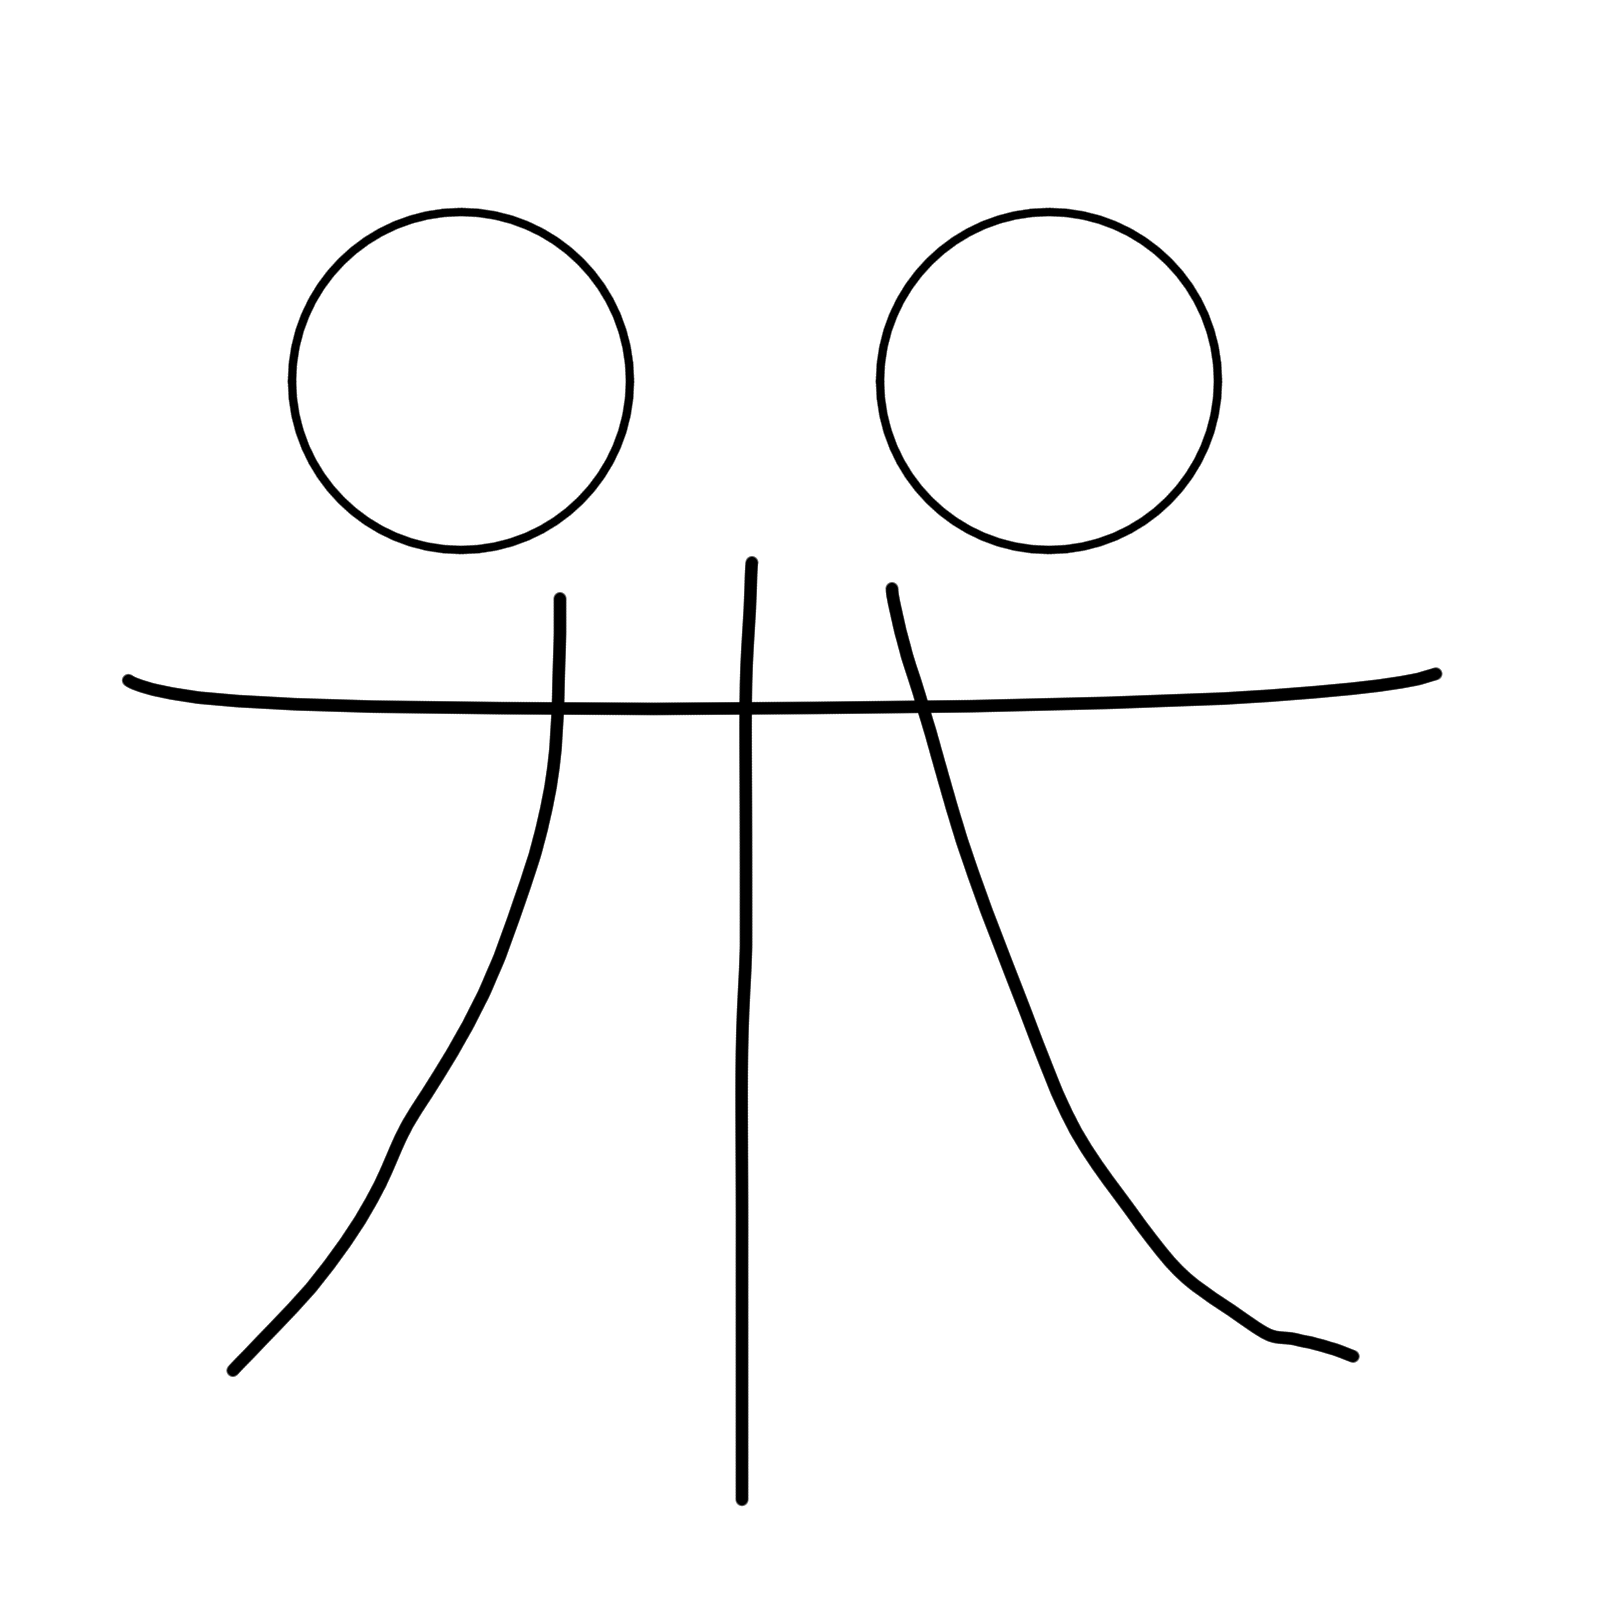
\includegraphics[width=\linewidth, height=25mm]{img/08keyframe}
    \end{minipage} &  
    \begin{minipage}{.28\textwidth}
      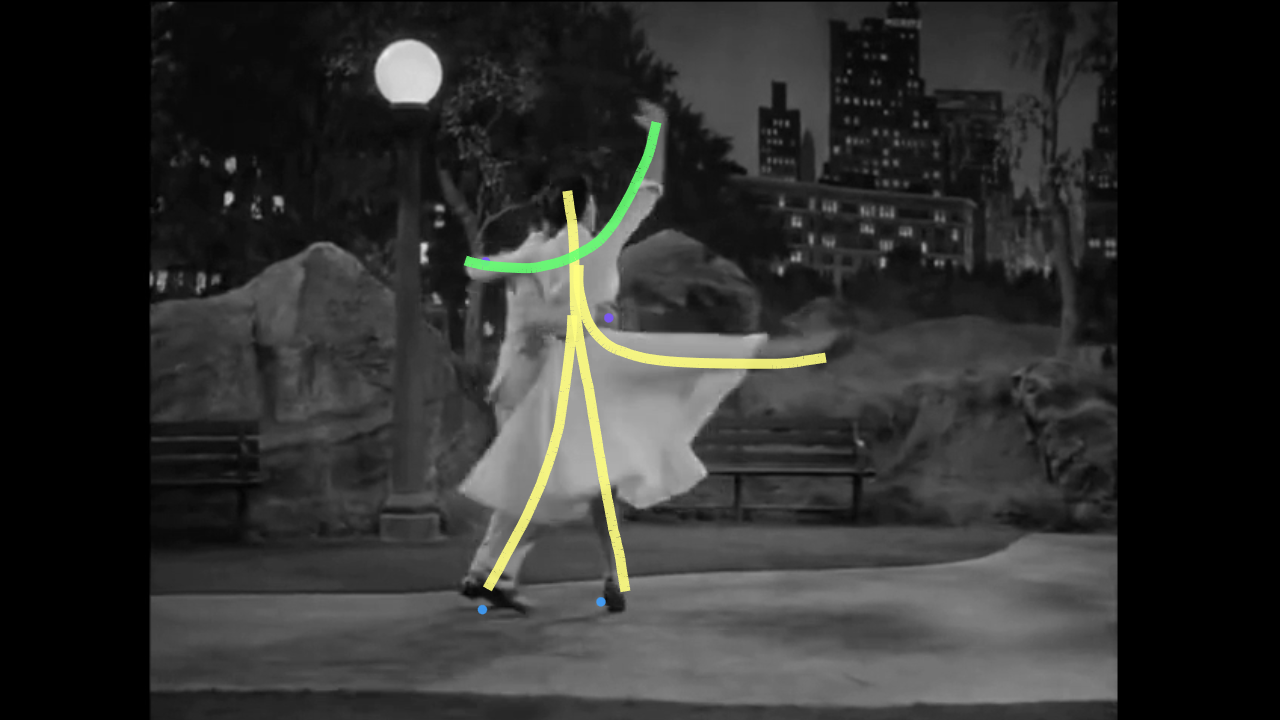
\includegraphics[width=\linewidth, height=25mm]{img/keyframe_case_8_(4)}
    \end{minipage}\\
	\begin{minipage}{.28\textwidth}
      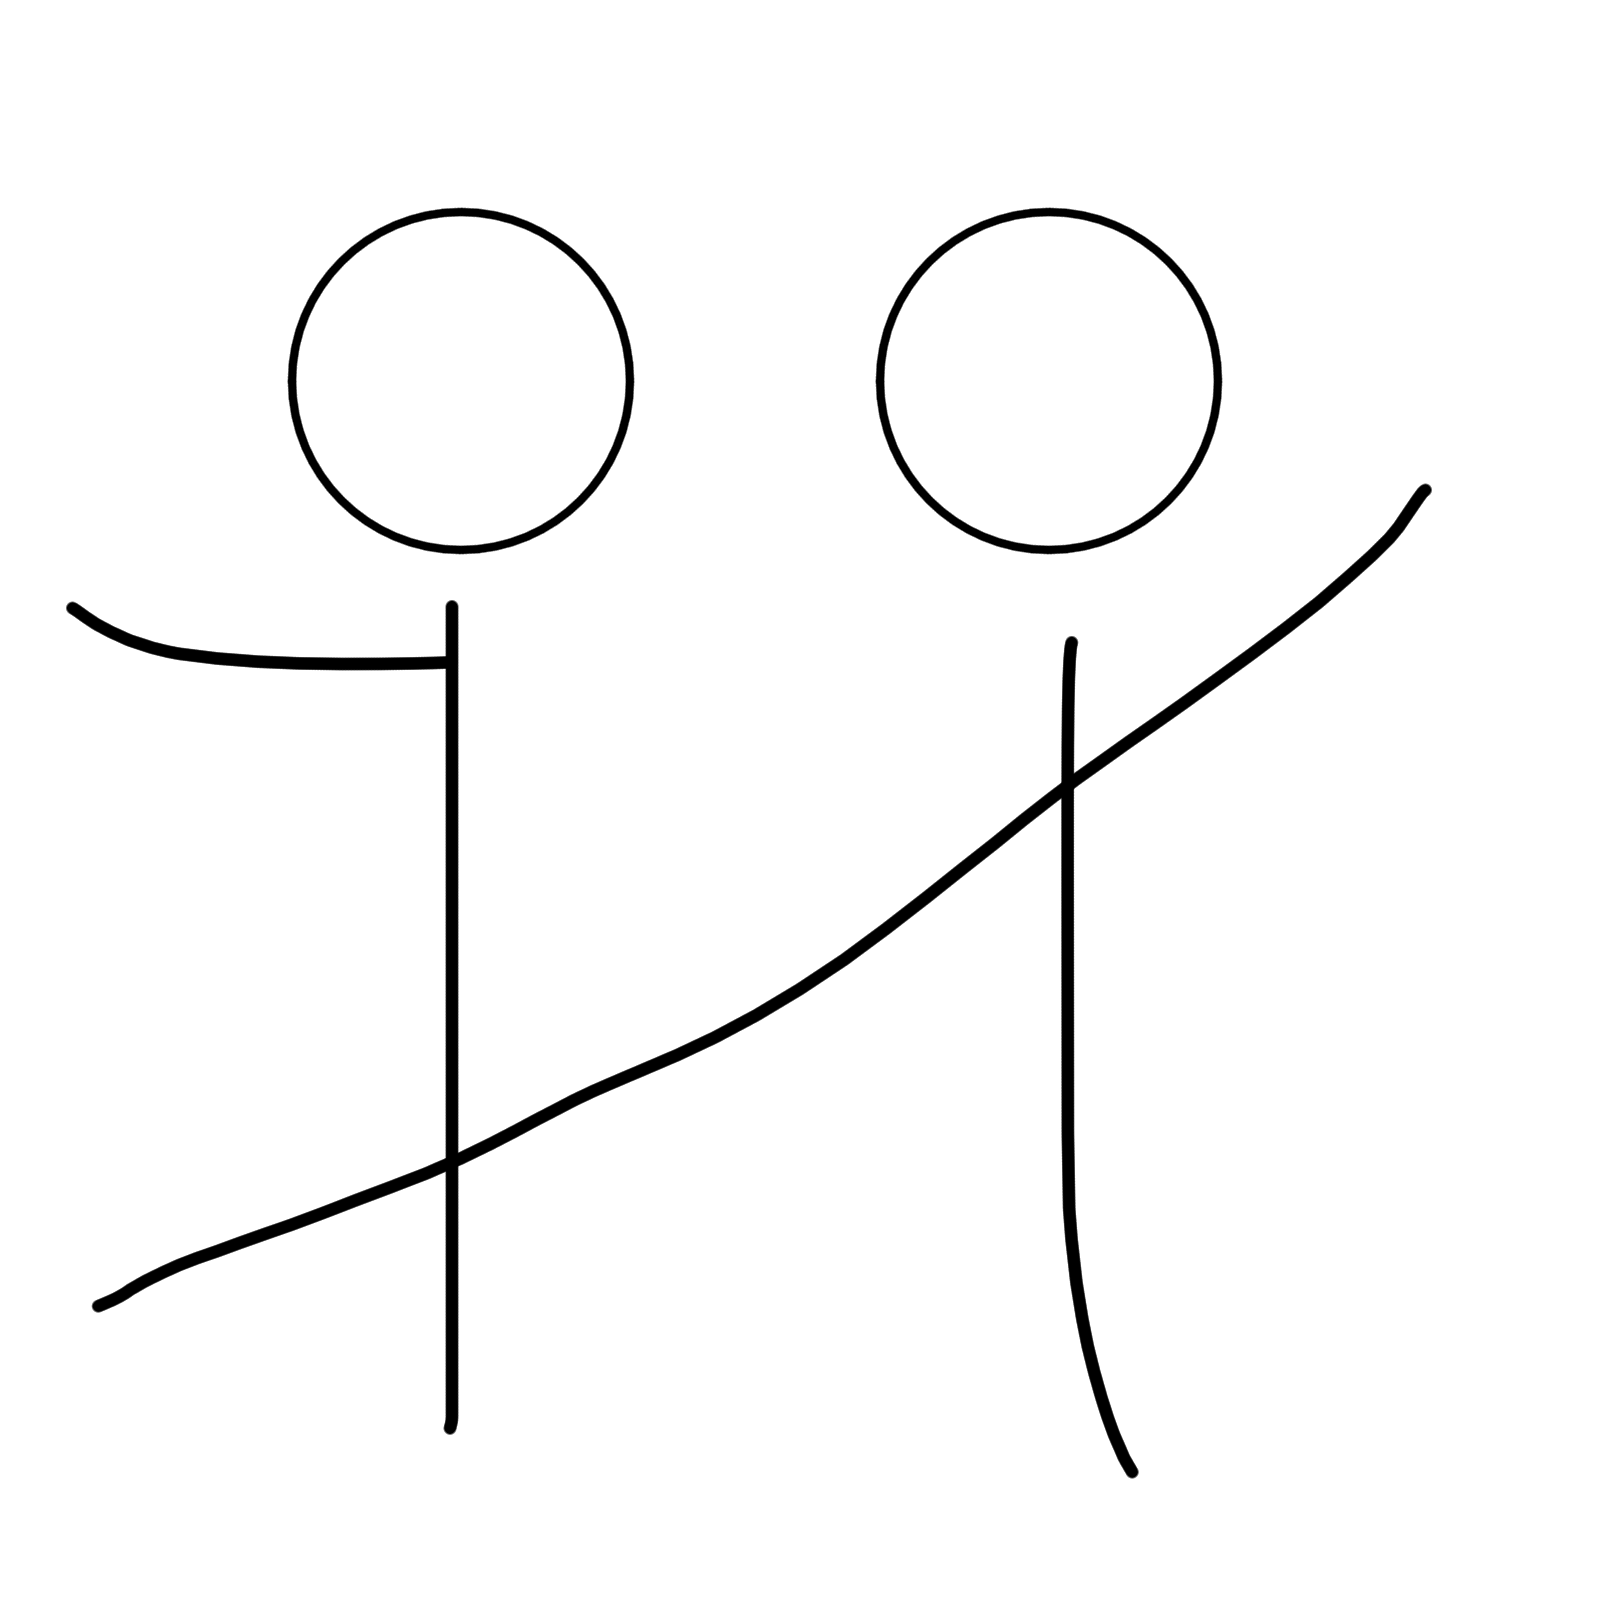
\includegraphics[width=\linewidth, height=25mm]{img/09keyframe}
    \end{minipage} &  
    \begin{minipage}{.28\textwidth}
      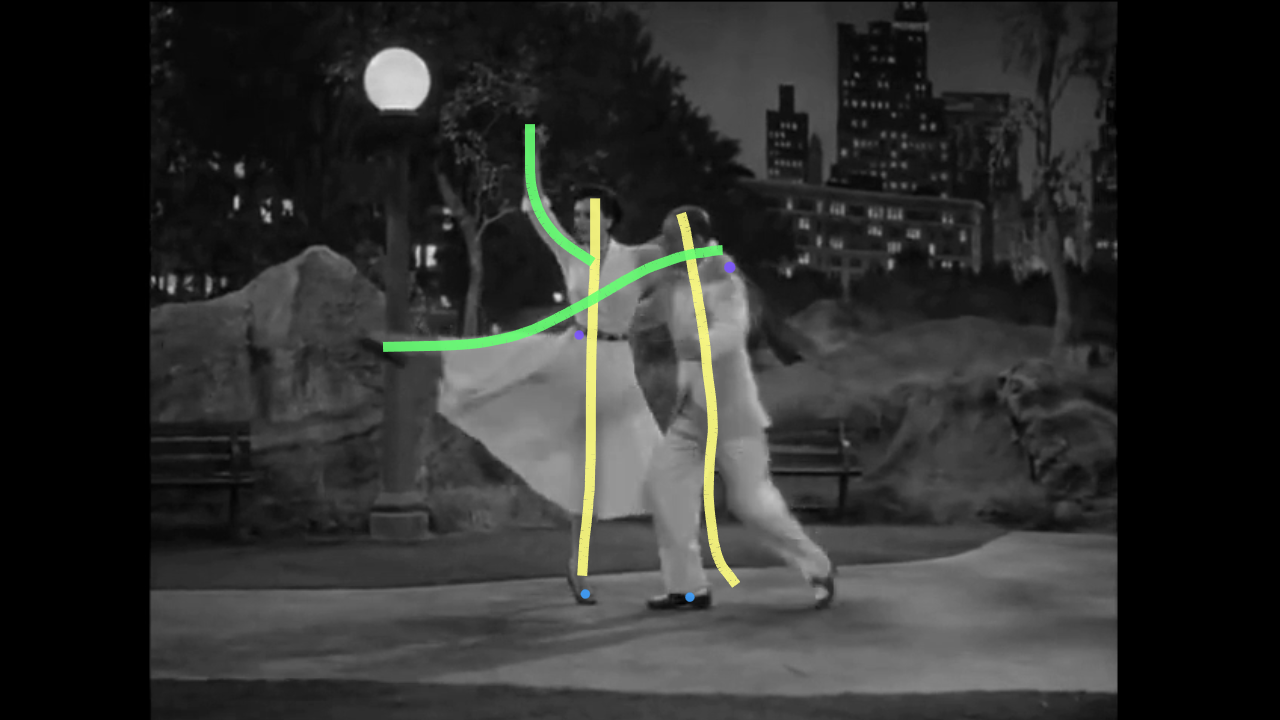
\includegraphics[width=\linewidth, height=25mm]{img/keyframe_case_9_(4)}
    \end{minipage}\\
	\begin{minipage}{.28\textwidth}
      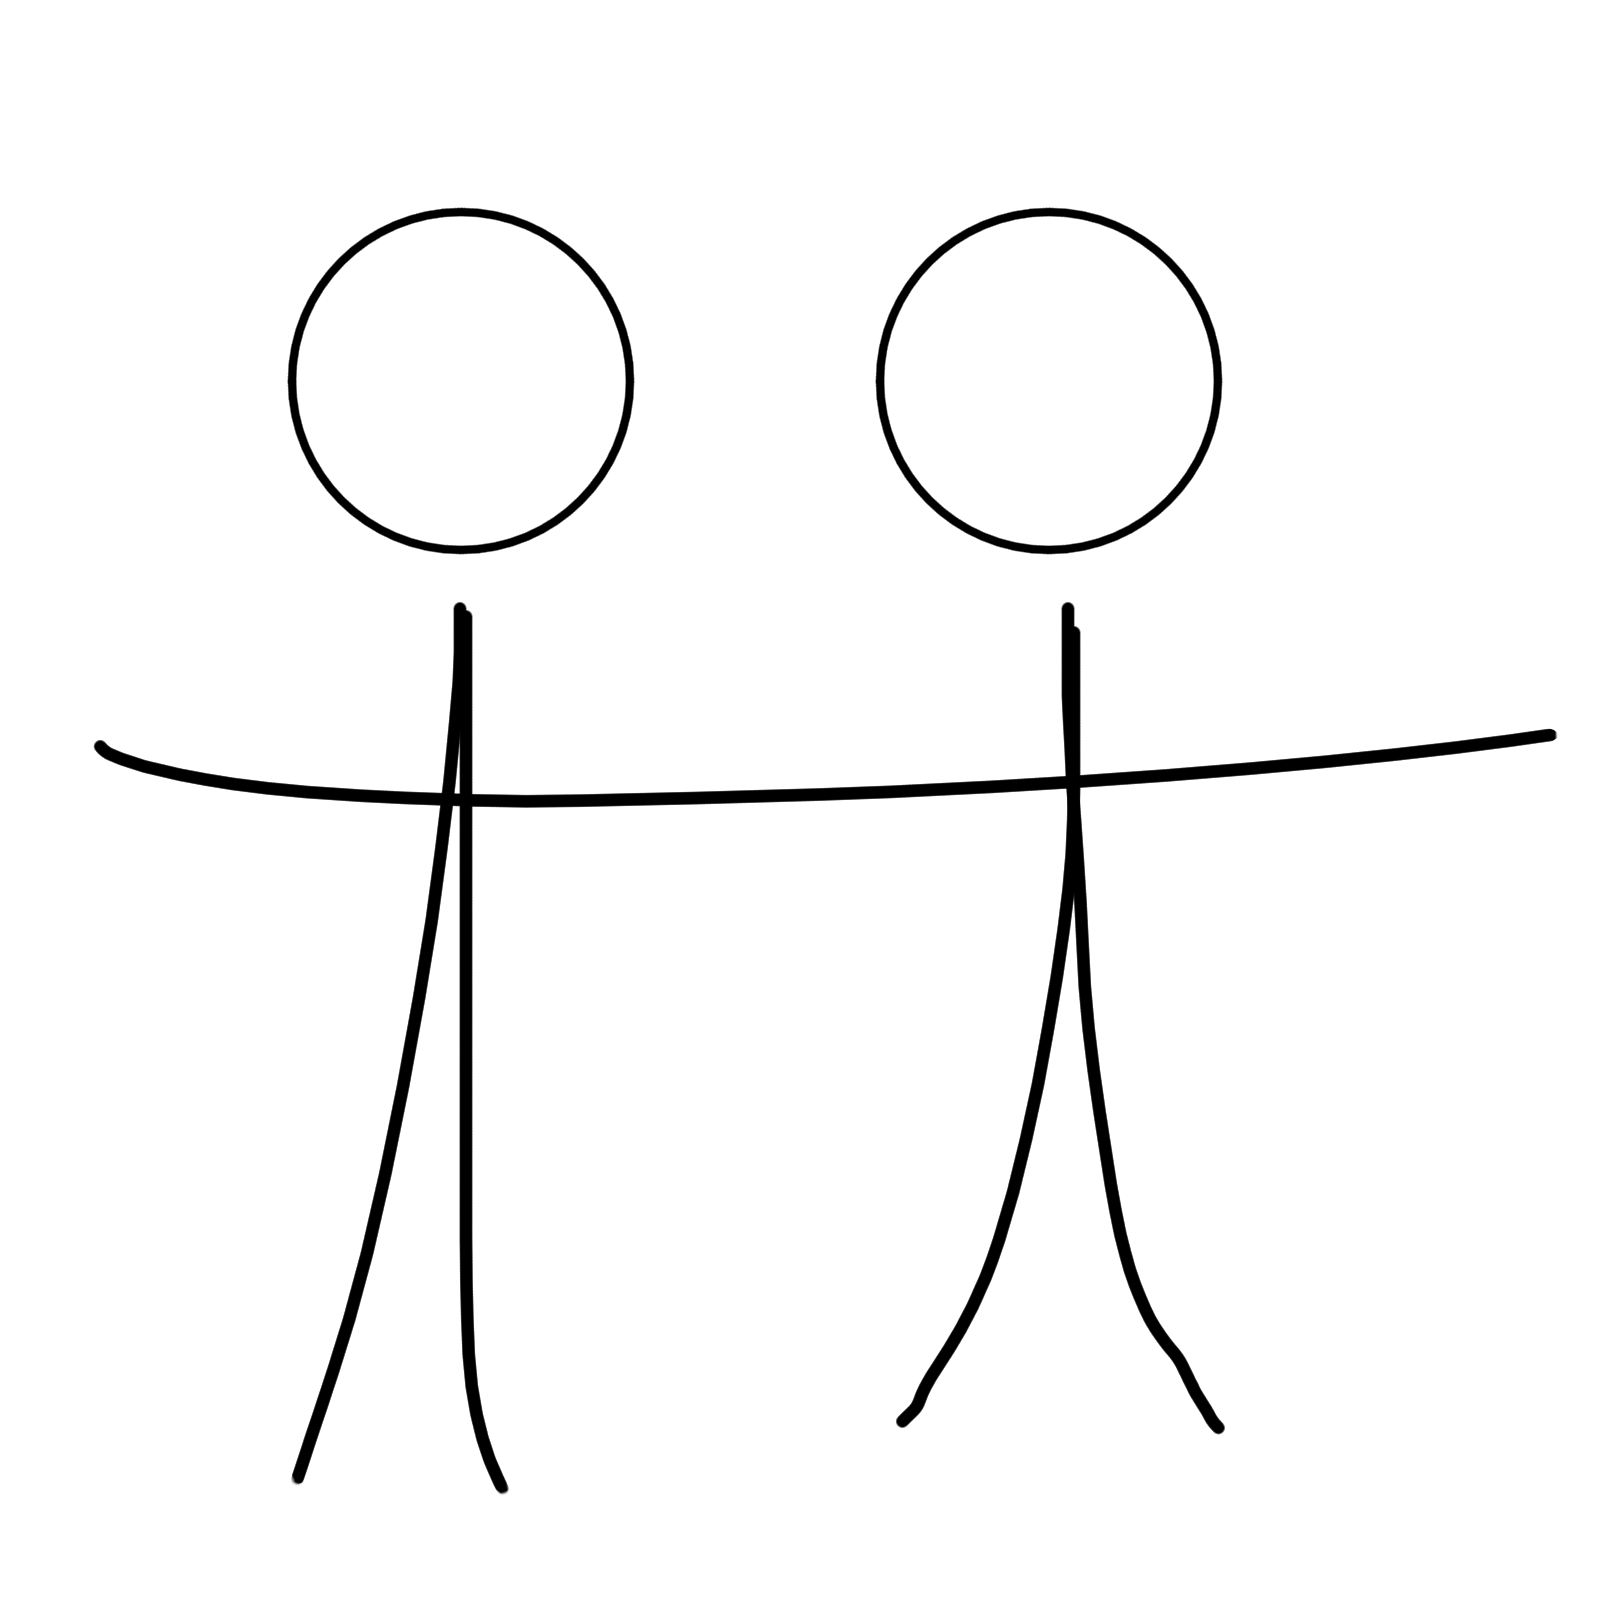
\includegraphics[width=\linewidth, height=25mm]{img/10keyframe}
    \end{minipage} & 
    \begin{minipage}{.28\textwidth}
      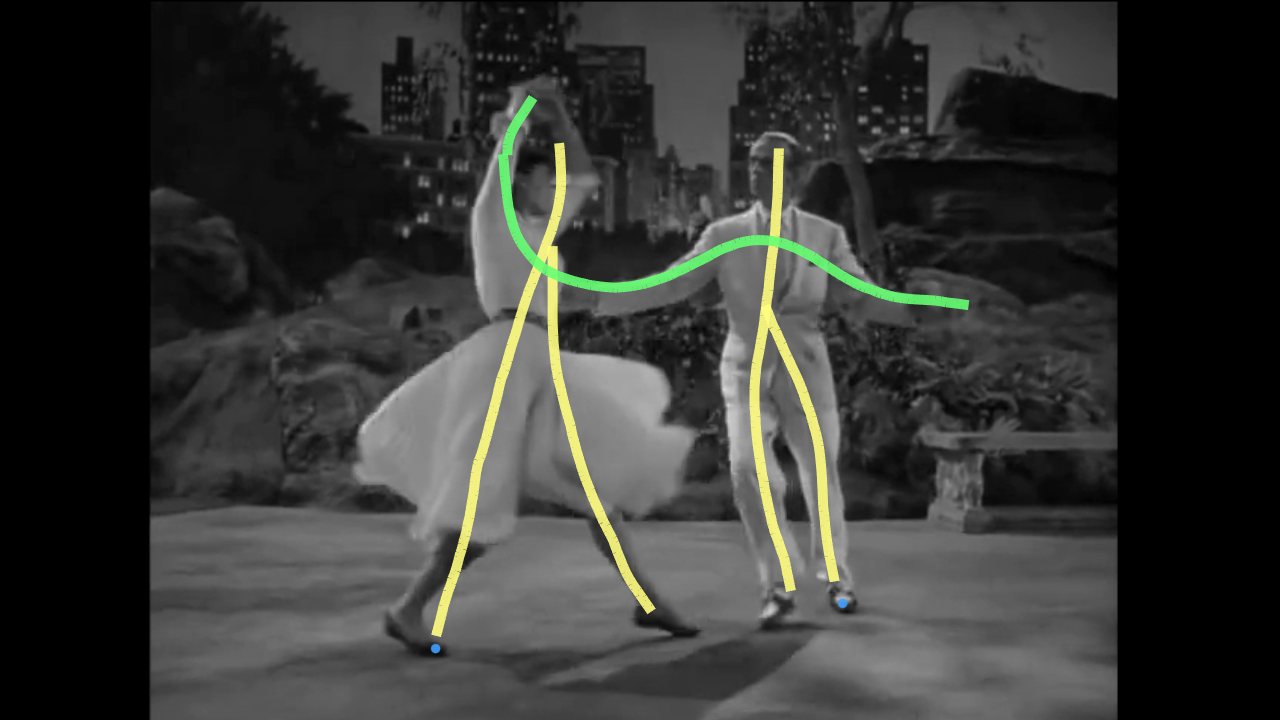
\includegraphics[width=\linewidth, height=25mm]{img/keyframe_case_10_(5)}
    \end{minipage}
\end{tabular}
\caption{Common LOA combinations and their corresponding examples in the video.}
\label{tab:combos}
\end{table}

\section{Merging Kinematic Trees}
Rather than changing the whole LOA concept and matching algorithm, we reduce the more complex problem of using LOAs on multiple characters to the original LOA problem and utilize the same iterative method to pose. At each keyframe, the kinematic trees of the two characters are to be merged in a consistent way that preserves the tree structure. Then this new structres is controlled by the new proposed lines of action.

From \citep{guay2015space}, since there is a viewing plane constraint on which the user draws the posing line, only one angle per joint has to be calculated to get from its current position to the target position. Starting from one end of the selected body line, local joint rotations are found using this equation:
\begin{equation}\label{eq:matching}
\theta_i(t) = \angle (Px_{i+1}(t) - Px_i(t), z_{i+1}(t)z_i(t)) 
\end{equation}
where $Px$ is the joint directed projected onto the viewing plane at time $t$ and $z$ is the drawn joint direction determined by the LOA. The current joint $i$ is the parent of joint $i+1$. Then the angles $\theta_i$ are applied to each joint to move it to the new pose. This method is fast and performs well. So instead of changing it, we merge kinematic trees of characters into one combined tree. 

Internally, both the tree and graph structures of characters' skeletons are stored. There is also another type of node called a ``separator'' node, which is purely virtual and acts as a sort of local root to allow for more body line options.

\begin{figure}[H]
\centering
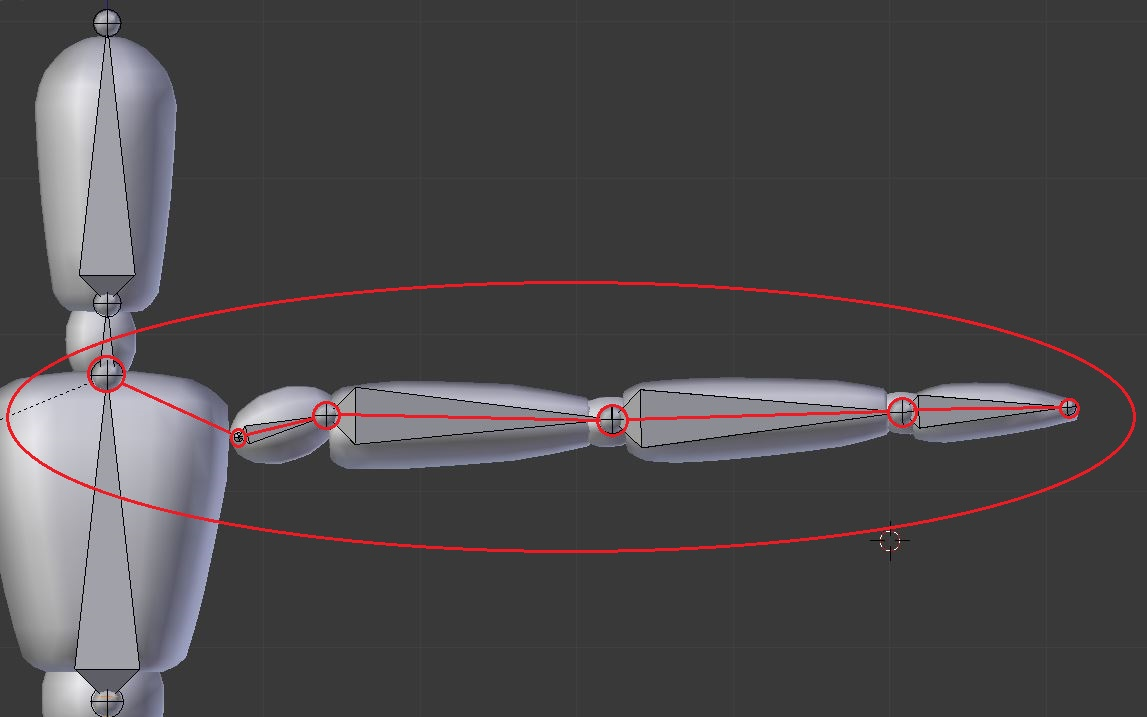
\includegraphics[scale=0.3]{img/shoulder}
\caption{In between the spine and the shoulder joints is a separator node, so the user can select only the arm as a body line.}
\end{figure}

\begin{algorithm}[H]
 \KwData{list of character hierarchies $h$, list of corresponding joints $pairs$}
 \KwResult{a single merged hierarchy}
 \If{$pairs$ is empty}
 {
  create a root node $mega\_root$\;
  \ForEach{hierarchy in $h$} 
  {
   make root of hierarchy a child of $mega\_root$\;
   \Return $mega\_root$\;
  }
 }
 \ForEach{correspondence in $pairs$}
 {
  \ForEach{joint in correspondence (2)}
  {
   go up hierarchy to find closest root or separator\;
   \If{roots are same}
   {
    connect joints into a $mega\_node$\;
    union the two nodes children\;
   }
   \Else{
	create a root node $mega\_root$\;
	make each joint a child of $mega\_root$\;
	reverse edges from each joint to their respective original nodes\;
   }
  }
 }
 enumerate cycles in using Johnson's algorithm (\citep{johnson1975finding})\;
 make each cycle into a new $mega\_node$\;
 \Return $mega\_root$\;
 
 \caption{The $merge\_hierarchies$ function.}
\end{algorithm}

A combined node is made by averaging frames (translation and rotation) of other nodes, effectively becoming a rigid body. A combined node made from a cycle averages all the frames of the nodes in the cycle with higher weight on the combined nodes within the cycle. A combined node made by connecting just two nodes averages the two frames and adds a virtual root. By combining nodes this way, we convert the two characters' trees into one, which is the goal.

A kinematic tree must be just that, a tree. It cannot have cycles and each node can only have one parent, so Johnson's algorithm is executed to find all simple cycles in the graph. From this all the nodes in the cycle are merged into its own combined node.

\subsection{Example}
\begin{figure}[h!]
	\centering
        \begin{subfigure}[b!]{0.6\textwidth}
        	\centering
                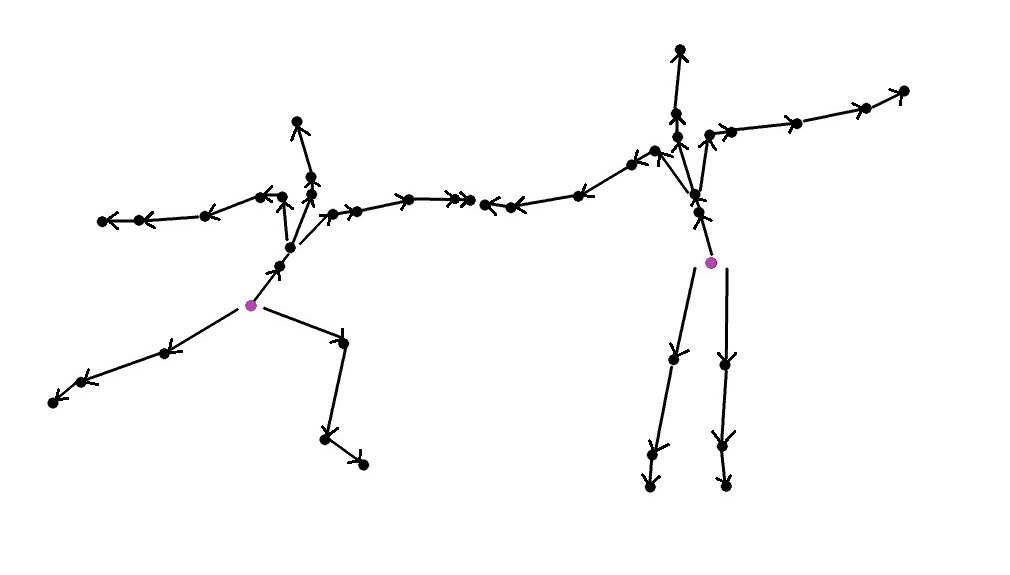
\includegraphics[width=\linewidth]{img/algorithm2}
                \caption{The two characters kinematic trees.}
        \end{subfigure}
        \quad
        \begin{subfigure}[b!]{0.6\textwidth}
        	\centering
                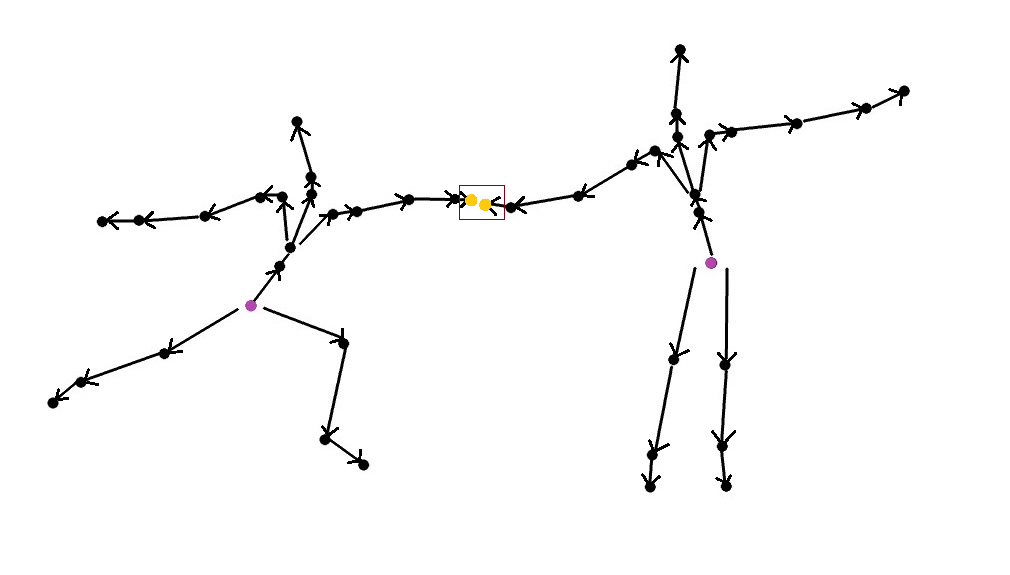
\includegraphics[width=\linewidth]{img/algorithm3}
                \caption{A pair of joints are selected to be combined and merge the two hierarchies. These particular nodes do not share a parent. So a virtual root needs to be created.}
        \end{subfigure}%
        \quad
        \begin{subfigure}[b!]{0.6\textwidth}
        	\centering
                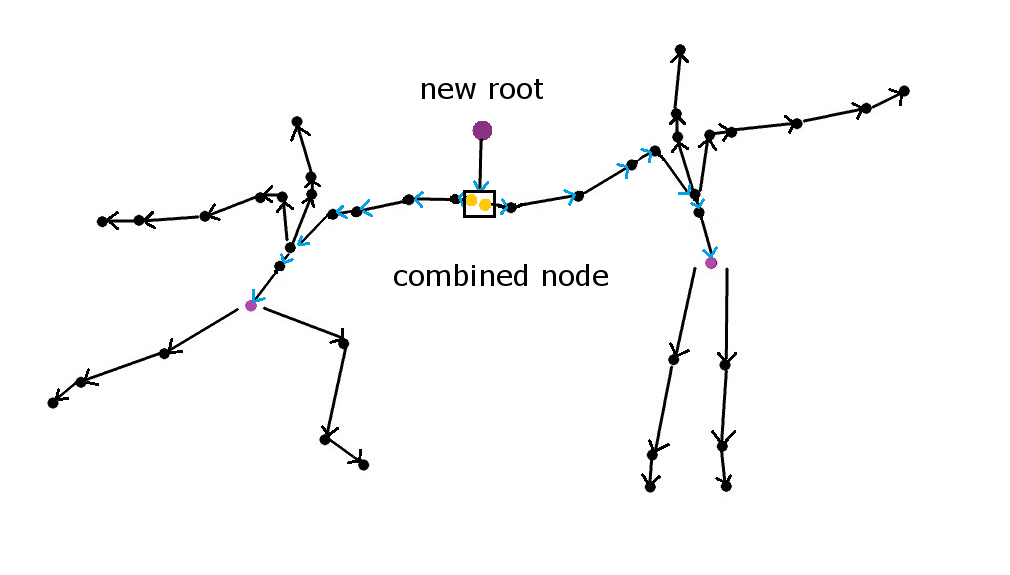
\includegraphics[width=\linewidth]{img/algorithm4}
                \caption{The new root is made the parent of the combined node. Then the edges to each original root are reversed to keep the data structure as a tree.}
        \end{subfigure}
    \caption{An example of the algorithm.}
	\label{fig:example}
\end{figure}

\section{Interface}
To select a body line for one character, the user clicks on which model they want either in the viewport or in the node list on the right hand side panel and activates annotation mode. Then they can press and hold shift and draw over the character, tracing the limb they want to select. A path is found between the two closest controllers to the endpoints of the LOA. If a path is found, the blue line shows what was finally selected. The red line is what the user drew and the green line shows a posing line.

\begin{figure}[h!]
	\centering
        \begin{subfigure}[b!]{0.45\textwidth}
        	\centering
                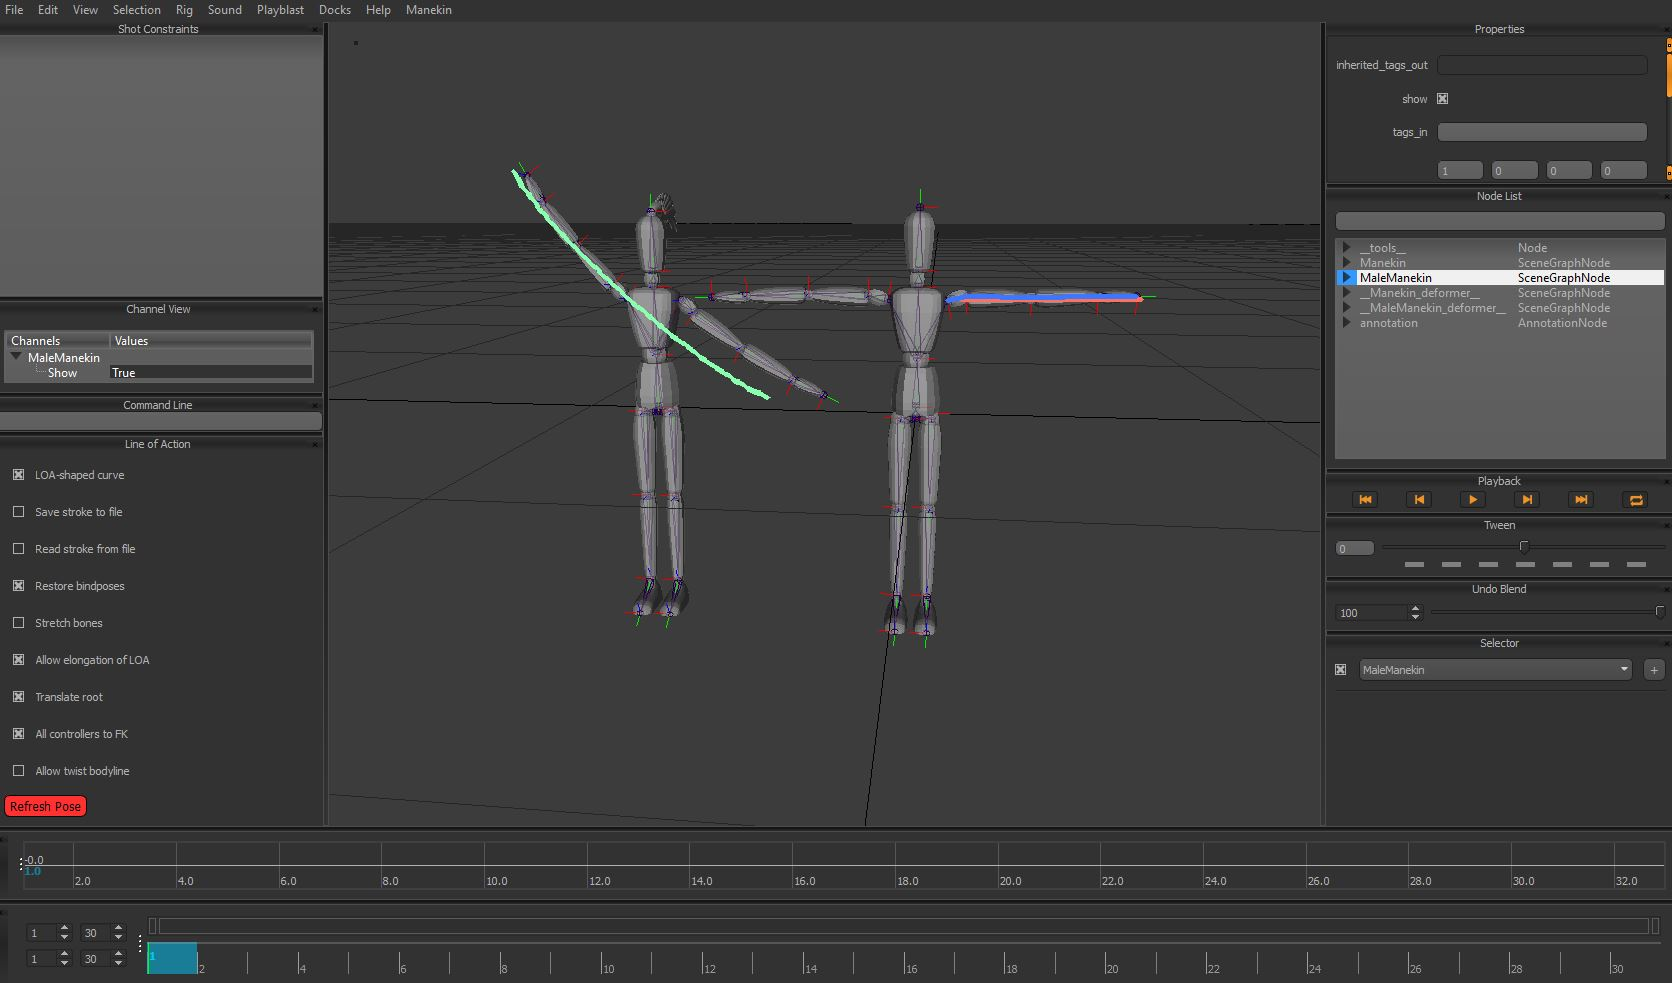
\includegraphics[width=\linewidth]{img/ui}
        \end{subfigure}
        \quad
        \begin{subfigure}[b!]{0.45\textwidth}
        	\centering
                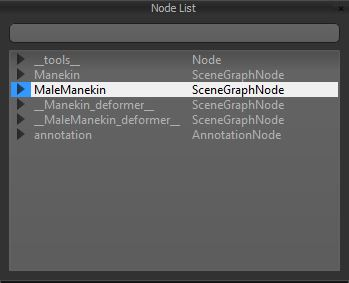
\includegraphics[width=\linewidth]{img/ui2}
        \end{subfigure}%
        \caption{Selecting a body line.}
	\label{fig:selection}
\end{figure}

To pose a character after a proper body line is selected, the user holds the control key while drawing a line with the mouse and \autoref{eq:matching} is used to match the body line to the LOA after the user releases the mouse. The green line shows the LOA. Note that now in the node list, all joints contained in the body line are selected, which allows the user to set keyframes using the LOA.

\begin{figure}[h!]
	\centering
        \begin{subfigure}[b!]{0.45\textwidth}
        	\centering
                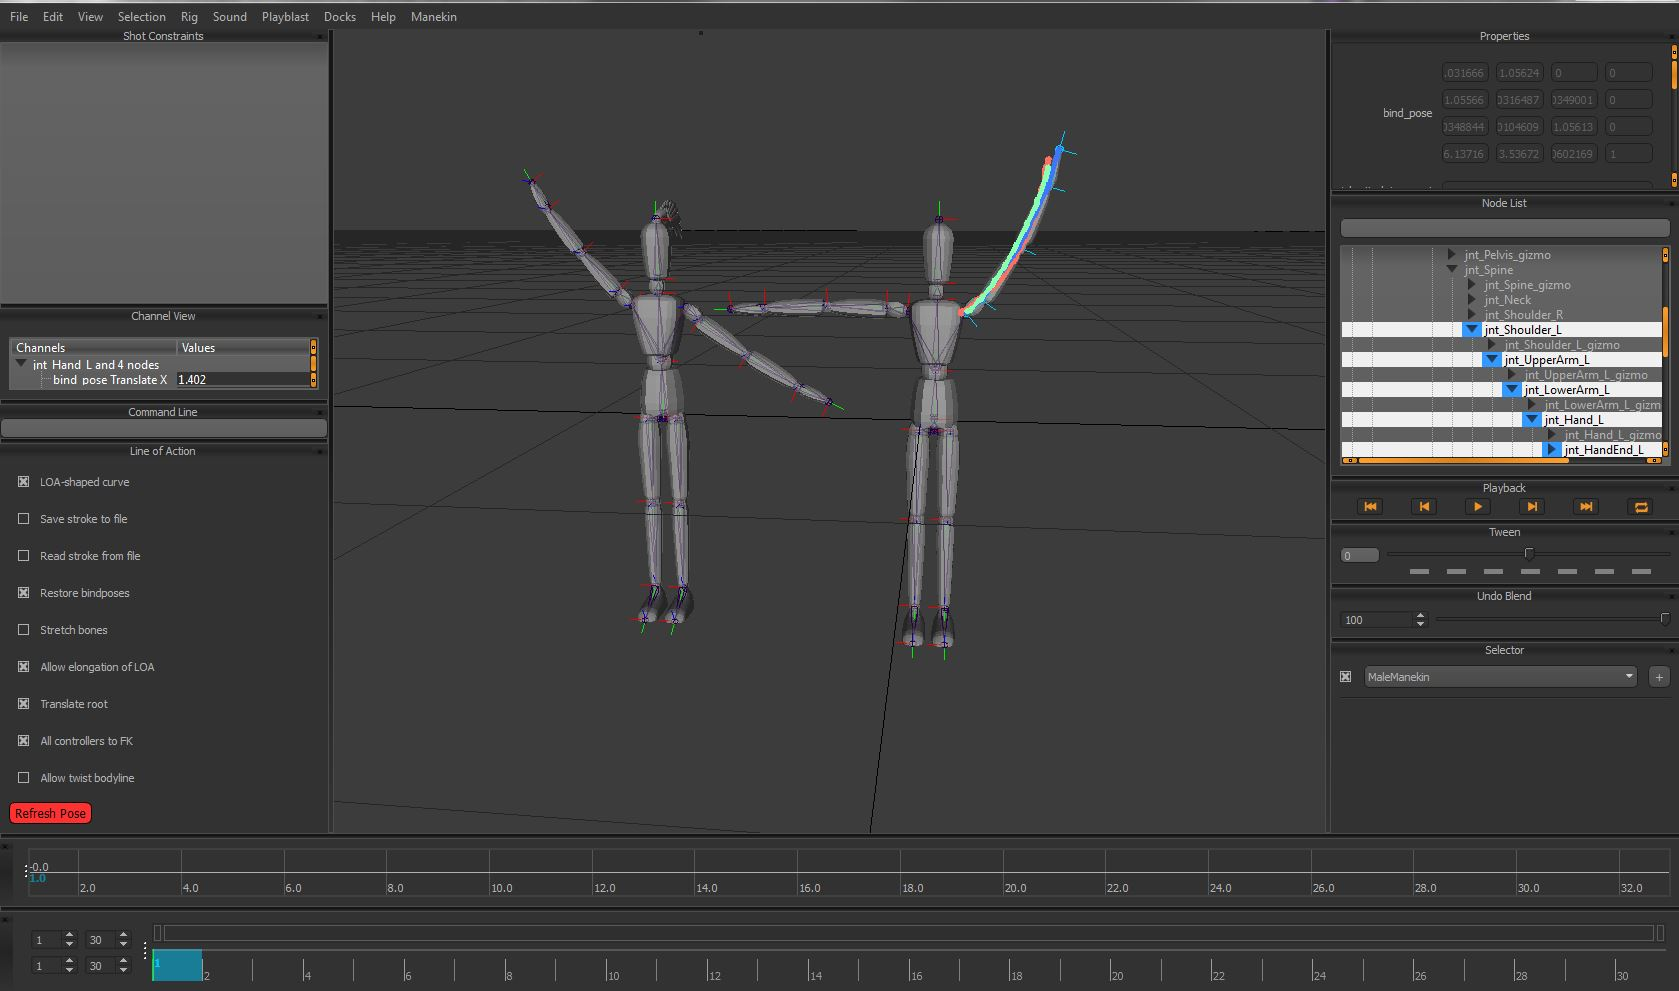
\includegraphics[width=\linewidth]{img/ui3}
        \end{subfigure}
        \quad
        \begin{subfigure}[b!]{0.45\textwidth}
        	\centering
                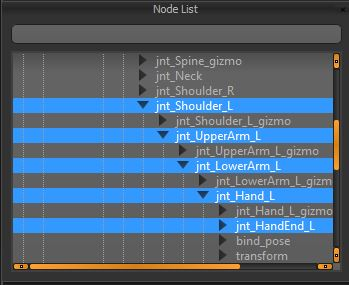
\includegraphics[width=\linewidth]{img/ui4}
        \end{subfigure}%
        \caption{Posing a body line.}
	\label{fig:posingbl}
\end{figure}

While in annotation mode, the user can then enter a sub-mode called joint selection mode. They can then click on pairs of joints and if valid, they will be highlighted in yellow. The user can deselect a joint before it goes into a pair, but when two joints are selected they are automatically put into a pair.

\begin{figure}[h!]
	\centering
        \begin{subfigure}[b!]{0.45\textwidth}
        	\centering
                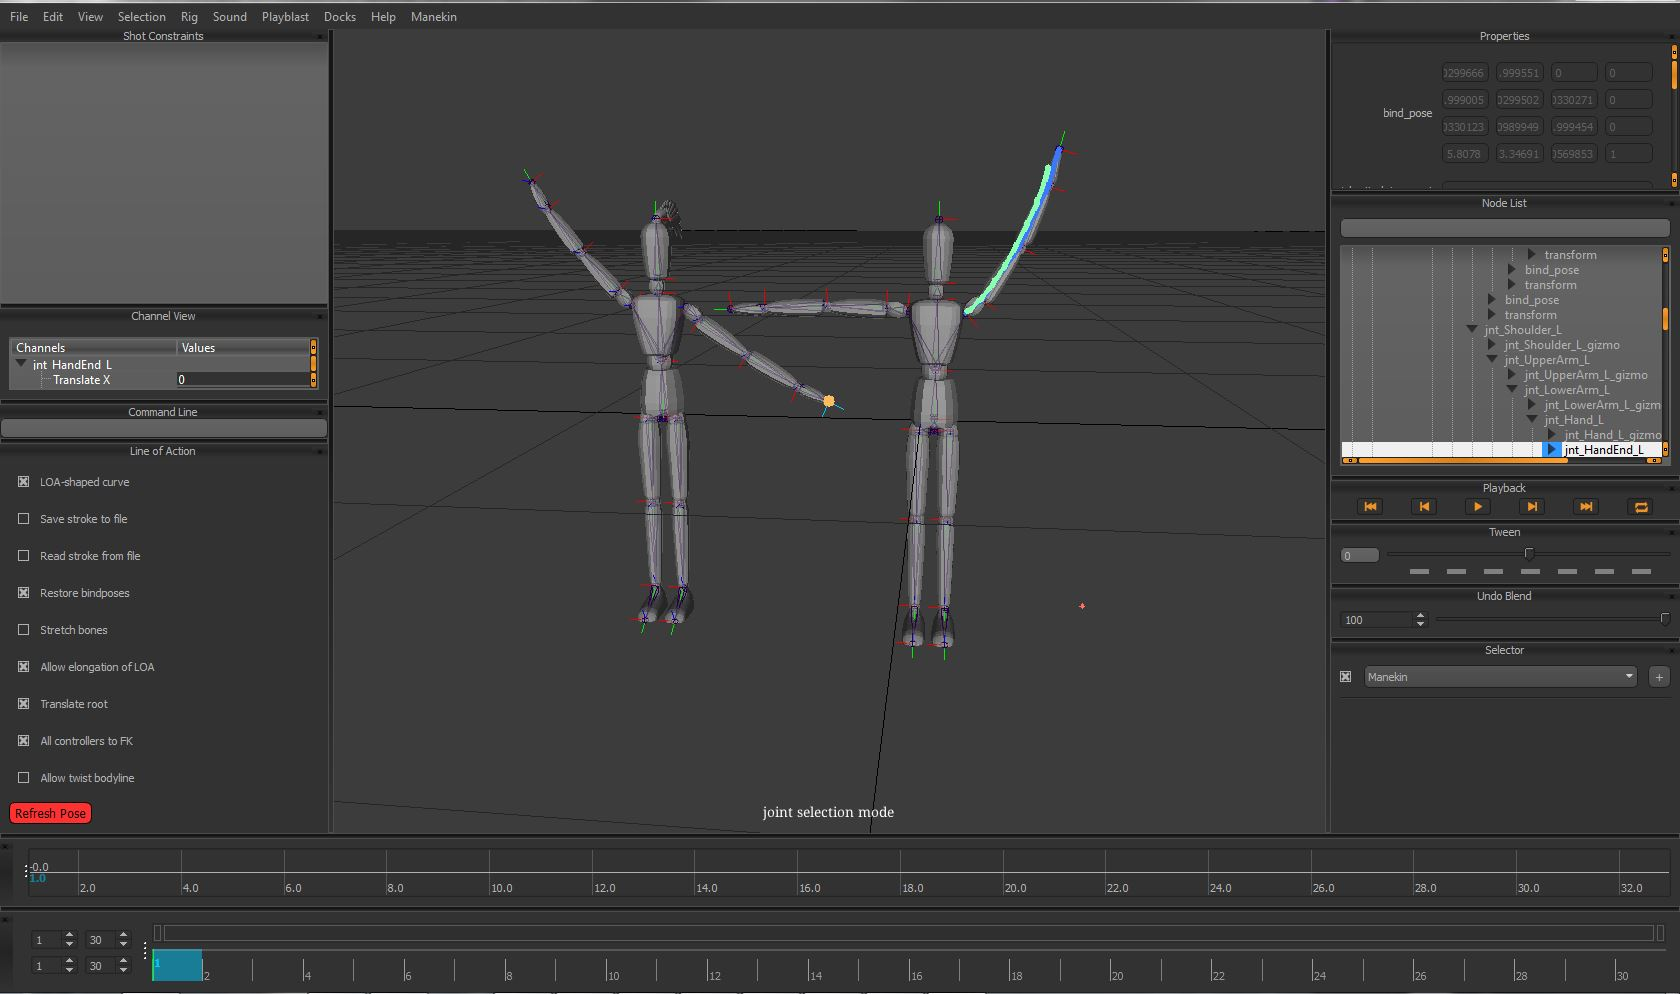
\includegraphics[width=\linewidth]{img/ui5}
        \end{subfigure}
        \quad
        \begin{subfigure}[b!]{0.45\textwidth}
        	\centering
                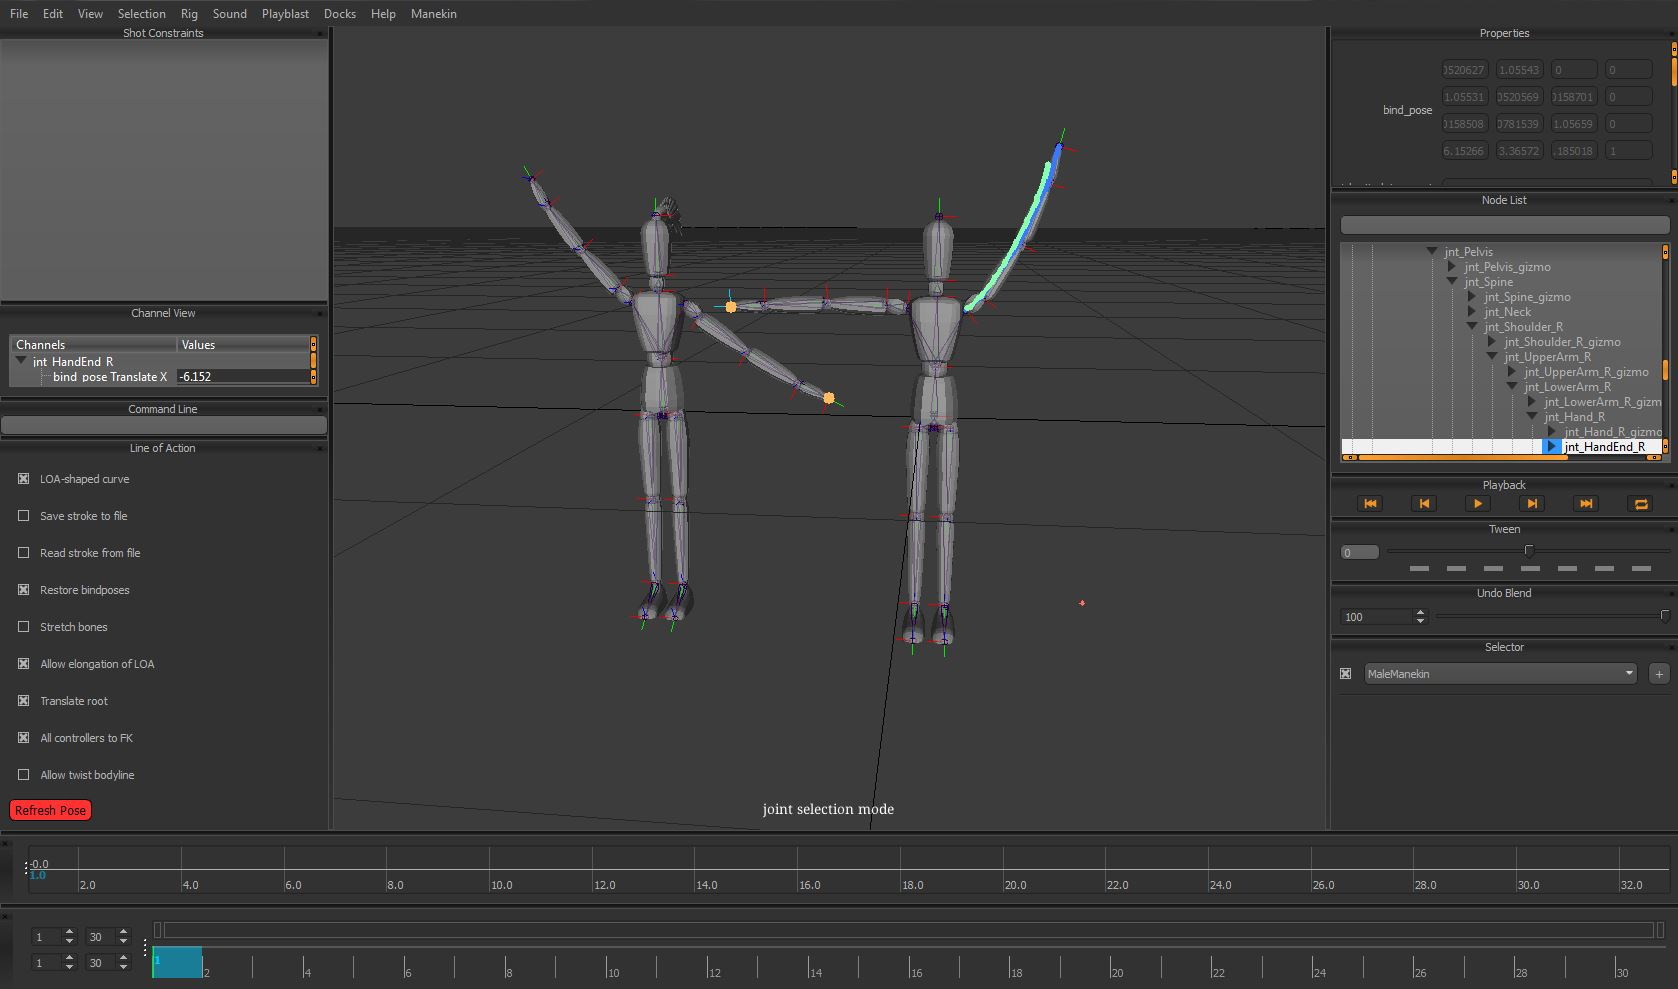
\includegraphics[width=\linewidth]{img/ui6}
        \end{subfigure}%
        \caption{Selecting a pair of joints to connect.}
	\label{fig:correspondence}
\end{figure}
